\documentclass[10pt,american]{article}
\usepackage{tgschola}
\usepackage{tgheros}
\renewcommand{\familydefault}{\rmdefault}
\usepackage[T1]{fontenc}
\usepackage{textcomp}
\usepackage[latin9]{inputenc}
\usepackage{babel}
\usepackage{varioref}
\usepackage{float}
\usepackage{booktabs}
\usepackage{calc}
\usepackage{pdfpages}
\usepackage{graphicx}
\usepackage[paperwidth=178mm,paperheight=178mm]{geometry}
\geometry{verbose,nomarginpar,tmargin=2cm,bmargin=2cm,lmargin=2cm,rmargin=2cm}
\usepackage[]
 {hyperref}

\makeatletter

\usepackage{datetime2}
\usepackage[os=win]{menukeys}
\renewmenumacro{\keys}[+]{shadowedroundedkeys}

\setlength{\parskip}{\medskipamount}
\setlength{\parindent}{0pt}

\makeatother

\usepackage{listings}
\renewcommand{\lstlistingname}{Listing}

\begin{document}
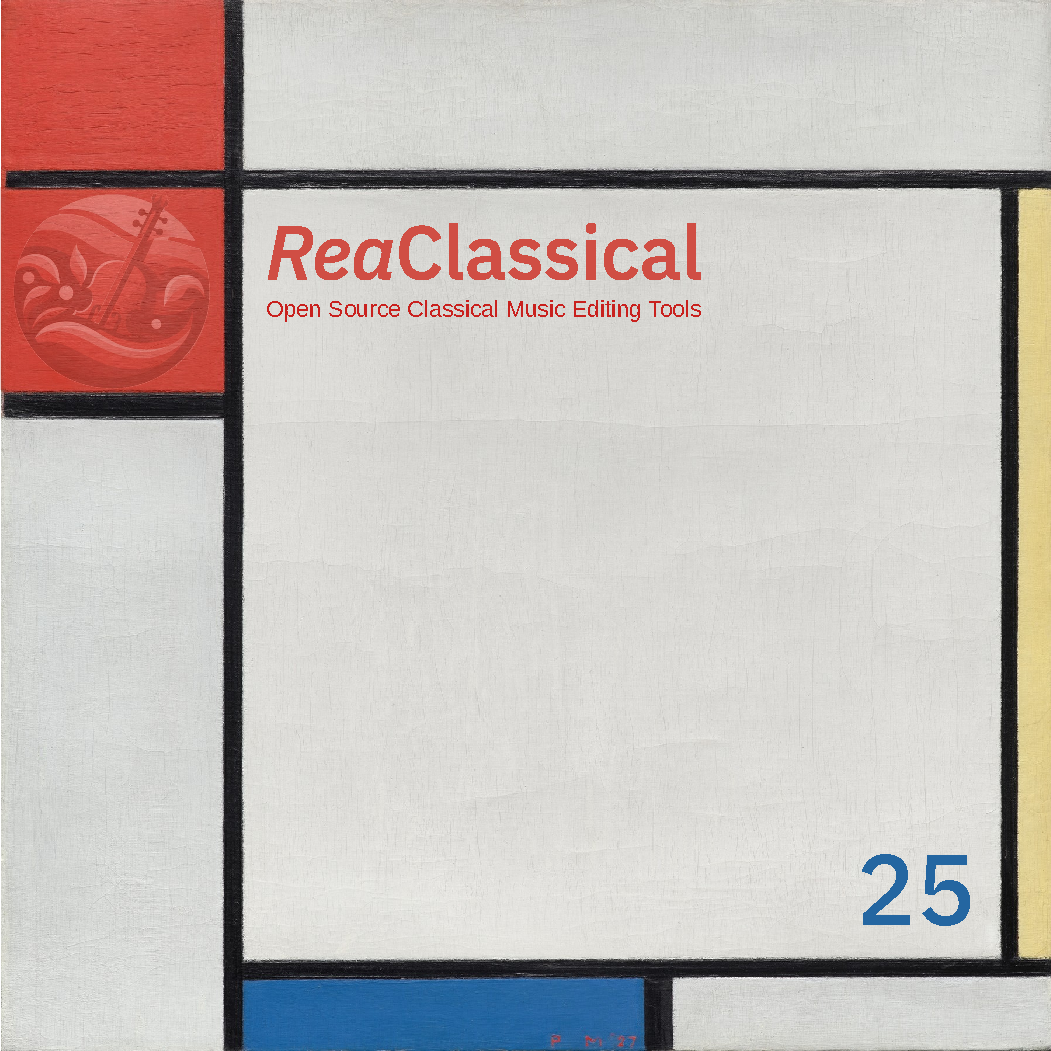
\includepdf{cover-front}
\author{}
\title{\textbf{The ReaClassical Manual}}
\date{Updated \today}
\maketitle
\begin{center}
This manual is released under the GNU Free Documentation License v1.3 \\
See
\href{https://www.gnu.org/licenses/fdl-1.3-standalone.html}{https://www.gnu.org/licenses/fdl-1.3-standalone.html}
\par\end{center}

\begin{center}
Copyright \copyright\ 2022--2025 chmaha \par\end{center}

\begin{center}
Cover art (adapted):\emph{}\\
\emph{Composition with Red, Yellow, and Blue} (1927) by Piet Mondrian\\
Downloaded from
\href{https://artvee.com/dl/composition-with-red-yellow-and-blue\#00}{Artvee}
\par\end{center}

\begin{center}
Typeset in \LaTeX using \TeX{} Gyre Schola font \par\end{center}

\vspace*{\fill}
\begin{center}
\begin{minipage}[c]{0.2\columnwidth}%
\begin{flushright}
\emph{As featured in}\thickspace{}\thickspace{} \par\end{flushright}%
\end{minipage}%
\begin{minipage}[c]{0.5\columnwidth}%
\href{https://www.soundonsound.com/techniques/source-destination-editing-reaclassical}{
\includegraphics[width=6cm]{user_guide_images/sos.jpg}}%
\end{minipage}
\par\end{center}

\vspace*{\fill}

\pagebreak{}

\vspace*{\fill}

\hyphenpenalty=10000

\emph{I sincerely appreciate your interest in ReaClassical. This project is a
labor of passion, driven by the desire to provide a robust and flexible tool for
musicians, composers, and sound engineers in the classical music world. Your
support, feedback, and contributions are vital to making ReaClassical better
with every update.}

\emph{Thank you for being a part of this journey. Whether you're just starting
with ReaClassical or have been using it from the beginning, your trust in this
tool inspires me to continue improving and innovating. I hope ReaClassical
enhances your classical music production workflow and empowers your creative
vision.}

\hyphenpenalty=50
\begin{flushright}

\includegraphics[scale=0.25]{user_guide_images/chmaha}
\par\end{flushright}

\vspace*{\fill}\pagebreak{}

\pagebreak{}

\tableofcontents{}\pagebreak{}

\part{Preliminaries }

\section{Introduction}

\noindent It is important to note that if you already own REAPER then the world
of classical editing including source-destination editing (aka 2-, 3-,
and-4-point editing), crossfade editing and more are available at no extra cost
to you via the freely available ReaClassical system. There's no need to spend
any of your hard-earned money on Sequoia, Pyramix or SaDiE in order to make
editing precise and efficient. As a classical engineer myself, I can say with
certainty that what I am about to share with you covers all my recording,
editing and mastering needs. Indeed, I couldn't return to the old way of working
at this point. Your mileage may vary and I'd love to hear from you if there are
functions that you feel might be missing. 

\section{Compatibility}

ReaClassical runs on any system that is compatible with REAPER (nine
architectures!). This includes 64-bit and 32-bit versions of Windows, MacOS and
Linux (including Raspberry Pi).

\section{Quick Start Guide}

For first-time users, the
\href{https://reaclassical.org/quick_start_guide.html}{quick start guide}
website is a great place to learn the basics about ReaClassical. Each section
covers major workflow areas and contains simple step-by-step instructions with
an accompanying short YouTube video for demonstration (no audio).

\section{This Manual}

This PDF manual serves as the official manual for ReaClassical. The latest
version is always available directly online or offline from within ReaClassical
by pressing \keys{H} (for `help'). The benefit of the offline version is that it
is always in sync with the version of the tools you are using. The structure of
the manual is designed to take the user through preliminary remarks, install and
update procedures for both ReaClassical and REAPER then a detailed look at
workflows from creating a project through to final render. After some brief
closing remarks, there follows the appendices (descriptions of all the
ReaClassical functions, keyboard shortcut guide, recommended free
mastering-grade plugins, system tweaks for all three major OSes, and, finally, a
manual install guide mainly for academic purposes).

I highly recommend doing a complete read of the manual and becoming very
familiar with appendices A and B.

\section{Website}

The website \href{https://reaclassical.org}{reaclassical.org} serves as the
entry point for new users. From here you can read about key features, donate to
the cause, read this PDF manual, installation instructions, navigate to the
ReaClassical community thread and more.

\section{REAPER Community}

The \href{https://forum.cockos.com/showthread.php?t=265145}{community thread}
plays an important role in the development of ReaClassical. Not only is it a
place for users to suggest feature requests and point out bugs but also discuss
more general classical music recording, mixing and mastering techniques. It also
serves as something of a development blog as I not only announce the regular
releases but also document the under-the-surface details for those that are
interested.

Relatively new is the \href{https://discord.gg/Gu2m9ccHGS}{ReaClassical Discord
server}. This is a great place for live support, general chat, proposing feature
requests, workflow discussion, and letting the community know about albums or
individual pieces you have created with the help of ReaClassical.

\section{Ways to Contribute}

The most important way users can contribute to the development of ReaClassical
is to actually use the tools! It makes me happy to know that engineers can make
whole professional-sounding and technically accurate masters from ReaClassical.
Another is to suggest features or let me know about bugs. You can either do this
on the \href{https://forum.cockos.com/showthread.php?t=265145}{thread} or via
the \href{https://github.com/chmaha/ReaClassical/issues}{Issues} page on the
ReaClassical GitHub. Finally, I'd be glad of any monetary donations. You can use
\href{https://www.paypal.com/donate/?hosted_button_id=PKJLC3E2UPW6C}{PayPal},
\href{https://liberapay.com/reaclassical/}{Liberapay} or
\href{https://donate.stripe.com/00g5mydzCftQdpeaEE}{Stripe} to do so. 

\section{Spread the Word!}

If you've enjoyed using ReaClassical in your projects, I'd be incredibly
grateful if you could mention it in your album booklets, social media video
descriptions, or anywhere you typically include session details. A simple
acknowledgment alongside your usual credits helps spread the word and supports
the continued development of the tool.

\section{Buy ReaClassical Merch}

Get print-on-demand ReaClassical merch like shirts, mugs, totes, pins, stickers
and more through my \href{https://www.teepublic.com/user/reaclassical}{TeePublic
store}!

\section{Source Code}

The source code for ReaClassical, the mastering grade `RC' plugins, this manual
and the website can all be found
\href{https://github.com/chmaha/ReaClassical}{here}. ReaClassical is
\href{https://www.gnu.org/licenses/gpl-3.0.html}{GPL-3.0} licensed.

\section{Development Style}

Due to working on GitHub and releasing the functions via ReaPack, I have the
ability to push bugfixes and new features very quickly into an existing
ReaClassical install. Often bugfixes happen within minutes or hours of receiving
the report. When I dream up new features, the development often happens in rapid
fashion over the course of a few days. However, now that ReaClassical has what I
consider a mature feature set, I foresee maintenance and occasional bugfixes
becoming more central to the process. This will give me more opportunity to work
on this documentation, a complete video tutorial series etc. Part of development
is also ensuring that ReaClassical continues to operate as expected with the
latest REAPER versions. That's not to say there won't be new features appearing!
As the REAPER developers add more new features, I will always check to see what
might be useful for ReaClassical. 

\section{Versioning Style}

ReaClassical currently uses YY.M.MICRO versioning (where M is a non-padded
month) to accurately reflect how current the software is. For example, 25.6.2
would indicate a June 2025 release with 2 further updates which might include
new features, improvements to existing functions, or bugfixes. 

\section{Tools and Languages}

ReaClassical works on top of \href{https://www.reaper.fm/}{REAPER}, the digital
audio workstation and utilizes \href{https://reapack.com/}{ReaPack} and
\href{https://www.sws-extension.org/index.php}{SWS Extensions}. ReaClassical
functions are coded using \href{https://www.lua.org/}{Lua}. The installers for
MacOS and Linux are shell scripts. The Windows installers are coded in
\href{https://go.dev/}{Go}. The ReaClassical and Quick Start Guide websites use
\href{http://getskeleton.com/}{Skeleton}. All coding is done either in REAPER's
ReaScript Development Environment, \href{https://code.visualstudio.com/}{vscode}
or \href{https://gedit-technology.github.io/apps/gedit/}{gedit} on Linux. The
manual is written in \LaTeX{} with the covers designed in
\href{https://www.libreoffice.org/}{LibreOffice} Draw. The ReaClassical splash
screen and banner are created in \href{https://www.gimp.org/}{GIMP}.

\section{Keyboard Shortcuts}

When providing keyboard shortcuts, this manual assumes Windows or Linux as the
operating system when modifier keys are used. MacOS users should use the typical
standard substitutions. If in doubt, open up the actions menu via keyboard
shortcut \keys{?} or by navigating to \menu{Actions > Show action list...} to
see the current assignments. For reference (from REAPER's own user guide), here
is a table of equivalent modifier keys:
\begin{center}
\begin{tabular}{cc}
\toprule 
\addlinespace
\textsc{PC (Windows or Linux) Key} & \textsc{Mac (MacOS) Key
Equivalent}\tabularnewline\addlinespace
\midrule
\addlinespace
\midrule 
Shift & Shift\tabularnewline
\midrule 
Control (Ctrl) & Command (Cmd)\tabularnewline
\midrule 
Alt & Option\tabularnewline
\midrule 
Windows & Control\tabularnewline
\bottomrule
\end{tabular}
\par\end{center}

\section{Changelog}

The changelog for ReaClassical functions can be found by double-clicking on the
ReaClassical package in ReaPack and navigating to the `History' tab. Whenever
you sync ReaPack via \menu{Extensions > ReaPack > Synchronize packages} or the
ReaClassical\_Updater function, this information should also appear
automatically. For all updates including those not related to the functions
themselves, a changelog can be found in the
\href{https://github.com/chmaha/ReaClassical/raw/main/release_notes.pdf}{release
notes}.

\pagebreak{}

\part{Installation \& Updates}

\section{Install}

\subsection{Easy Complete Portable Installation (recommended)}
\begin{enumerate}
\item Follow the installation instructions
\href{https://github.com/chmaha/ReaClassical/blob/main/install_instructions.md}{here}
or in the `Installation \& Update' section of the
\href{https://reaclassical.org/quick_start_guide.html}{Quick Start Guide}.
Simply run where you would like the ReaClassical folder to be created. 
\item Start REAPER/ReaClassical.
\item Follow the update instructions \vpageref{subsec:Updating} to get the
latest and greatest versions of the ReaClassical functions, toolbar and keymap.
\end{enumerate}
Note that if the ReaClassical folder already exists, the installer will
automatically add a unique suffix to ensure nothing is overwritten.

\subsection{Just The Scripts and Plugins?}

Install both \href{https://reapack.com/}{ReaPack} and latest
\href{https://www.sws-extension.org/download/pre-release/}{bleeding edge SWS
Extensions} if you haven't already. 

Import my
\href{https://github.com/chmaha/ReaClassical/raw/main/index.xml}{index.xml} into
ReaPack (see the
\href{https://reapack.com/user-guide\#import-repositories}{ReaPack user guide}
if you are unsure how) and search for `ReaClassical' for the ReaClassical
metapackage and `RCPlugs' for the classical jsfx plugins. Note that out of the
box this does \emph{not} give you the full benefits of ReaClassical which
include keyboard shortcuts, custom toolbar etc but does include ReaClassical
themes and a project template which you should use when doing classical editing.
It's an easy way to start if you are already familiar with ReaPack and SWS and
want to check out source-destination editing etc. Note that you \emph{do} need
SWS installed for the functions to work as expected. You can follow the update
instructions \vpageref{subsec:Updating} to grab the custom toolbar and keymap
but please heed the warning about using the ReaClassical\_Updater function as
answering 'yes' to either of the questions will overwrite configuration files.

\subsection{Manual Installation \& Tweaks}

\noindent For a manual installation (ideally for educational value only or if
you already have a heavily-customized REAPER setup and wish to add all or just
parts of ReaClassical) see Appendix E.

\section{Update}

\subsection{\label{subsec:Updating}Updating an Existing ReaClassical Portable
Install}

To update just the functions, use \menu{Extensions > ReaPack > Synchronize
packages}. To update the functions and also update/reset the custom toolbar and
keymaps to be in line with a standard ReaClassical portable install, run the
handy ReaClassical\_Updater function via \keys{\shift+U} . This will sync
ReaPack to get the latest ReaClassical functions then offer to overwrite your
toolbars and keymaps with ReaClassical portable install defaults. \textbf{DON'T
do this if you have your own custom toolbars or keyboard shortcuts as they will
be overwritten! }However, as of 24.8.7 any files will first be backed up (e.g.
\emph{reaper-kb.ini.backup}). Obviously if you run the updater twice before
recovering them you will lose your original files.

\subsection{Updating REAPER}

Simply use the shortcut \keys{\ctrl+U} to open the REAPER update utility.

\begin{figure}
\begin{centering}
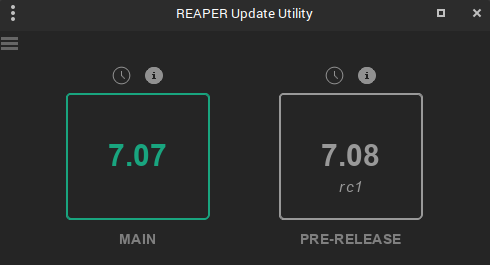
\includegraphics[scale=0.5]{user_guide_images/reaper_update_utility}
\par\end{centering}
\caption{REAPER Update Utility}

\end{figure}

Either click on the main or pre-release version you are interested in or click
on one of the clock icons to select from previous releases. Despite the REAPER
developers having a track record of excellent compatibility across even major
versions, I recommend sticking with the tested version of REAPER noted
\href{https://raw.githubusercontent.com/chmaha/ReaClassical/main/tested_reaper_ver.txt}{here}
to minimize any issues of compatibility.

\pagebreak{}

\part{ReaClassical Workflows}

\section{Creating \& Setting Up a Project}

When you start REAPER/ReaClassical from a default portable install, you'll see
an empty project with ReaClassical project defaults. The first thing you should
do is save it via \keys{\ctrl+S}.

\subsection{Theme}

The ReaClassical theme is loaded by default. It looks almost exactly like the
default REAPER theme. If you'd like to switch to one of several other custom
themes, you can do so via \menu{Options > Themes}. `ReaClassical Light' is
similar to the default but uses lighter waveforms and peak edging. The two
`WaveColors' themes apply coloring only to the waveforms with option for dark or
light item backgrounds.

\subsection{Project Settings}

You can open the project settings by pressing \keys{P} (for `Project Settings')
You shouldn't need to change any settings here. By default, render resampling is
set to the highest quality using r8brain free. Media is saved to a `media'
subfolder. The default recording format is 24-bit wave files but you can set to
32-bit float if using a portable recorder with that capability. Video frame rate
is set to 75 to align with the number of frames per second for an audio CD. You
can, of course, fill in the `notes' section with a title, author and notes as
desired.

\begin{figure}
\begin{centering}
\includegraphics[scale=0.5]{\string"user_guide_images/project prefs\string".png}
\par\end{centering}
\caption{REAPER Project Settings }

\end{figure}


\subsection{Audio Settings}

Click on the audio information in the top right of the window or via \keys{O}
(for `options') navigating to \menu{Audio > Device}. These settings are
operating system dependent. Choice of blocksize etc is also dependent on need
and how modern and/or optimized your system is. For general microphone setup,
device and recording settings specifically for classical music etc I recommend
referring to one or more of the following: 
\begin{itemize}
\item \emph{Classical Recording: A Practical Guide in the Decca
Tradition}\textsc{ }by Haigh, Dunkerley \& Rogers
\item \emph{Recording Orchestra and Other Classical Music Ensembles} by Richard
King
\item \emph{Recording Classical Music} by Robert Toft
\item For a more detailed look at mastering (for any genre of music), I highly
recommend \emph{Mastering Audio: The Art and the Science} by Bob Katz. 
\end{itemize}

\subsection{ReaClassical Project Preferences}

Pressing \keys{F5} brings up the ReaClassical Project Preferences dialog. The
first line sets the crossfade length in milliseconds for all source-destination
editing. The next three lines are for
\href{https://en.wikipedia.org/wiki/Disc_Description_Protocol}{DDP} creation.
The defaults are for a 200ms track offset (to account for older CD players that
couldn't play audio immediately after a track search), the INDEX0 length in
seconds for when to start a CD player `countdown' display to the next track (a
fun visual trick that is, of course, completely irrelevant for purely digital
releases) and, finally, the album lead-out time in seconds (essentially the time
on a car CD player before the disc returns to the beginning again). There is a
setting for the Prepare Takes function to either use the old random coloring
method or the newer color scheme that uses blues for destination material and
greens for source material. The user can change the checking range (distance
beyond an item edge/fade or crossfade) when placing destination IN and OUT
markers. Setting to 0 would just check if the marker would be placed
\emph{inside} a item fade or crossfade. If the reference track is set as overdub
guide, it will be audible during classical take recording and auditioning which
is extremely useful for overdub recording of material after the main session
such as a symphonic organ part or narration. Next, you can set
\keys{1},\keys{2},\keys{3}, and \keys{4} to add markers at the mouse hover
position vs edit cursor. In this mode, you can also enter the fade editor by
hovering of the right-hand items of a crossfaded pair and pressing \keys{F}. You
can set the custom playback rate when auditioning via \keys{\shift+A}. Next
there are two settings associated with CUE file production -- year of production
and audio file type. Finally, you can enable a floating destintion group which
shifts position based on the active source group. There will be more on these
settings in subsequent sections of the manual. If you are unfamiliar with these
concepts, I recommend a quick internet search! If in doubt, just use the default
values. It is worth noting that these preferences are set per project.

\begin{figure}
\begin{centering}
\includegraphics[scale=0.5]{\string"user_guide_images/RC Prefs\string".png}
\par\end{centering}
\caption{ReaClassical Project Preferences}
\end{figure}


\subsection{Choice of Workflow}

The choice between what I refer to as `vertical' or `horizontal' workflows will
depend somewhat on the complexity of the project. For a quick editing session
of, say, a choral piece or short self-standing orchestral piece, a horizontal
approach will suffice. For a well-drilled ensemble recording session, I can
recommend using the vertical approach. Many classical engineers enjoy using a
horizontal approach for recording (potentially the least disruptive and making
use of the Take Counter window \keys{Ctrl + \return}) and then either sticking
with that for editing (also taking advantage of the extremely useful Find Take
\keys{\return} and Jump to Time \keys{\tab} functions) or, depending on the
number of takes, converting to a vertical workflow. Frankly, there are benefits
to both routes, and in the end, it simply comes down to personal preference.

\begin{figure}
\begin{centering}
\includegraphics[scale=0.5]{\string"user_guide_images/take counter\string".png}
\par\end{centering}
\caption{Take Counter }

\end{figure}

\begin{figure}
\begin{centering}
\includegraphics[scale=0.5]{\string"user_guide_images/find take\string".png}
\par\end{centering}
\caption{Find Take }

\end{figure}


\subsubsection{Vertical Workflow}

In this approach, the source and destination track groups are aligned vertically
so that the user doesn't have to shuttle back and forth in the arrange window
for placing source-destination markers. 

\textbf{When Recording material:} To begin with a vertical workflow, you could
actually use a horizontal workflow approach \keys{F7} to set up just a single
group and record left to right. After recording is complete, and you are ready
for editing, you could convert to a vertical workflow via \keys{F8}.
Alternatively, you can press \keys{F8} for project creation and start
immediately with a vertical setup with one `destination' group and six `source'
groups. In either setup, and whether recording or importing, simply type in the
total number of stereo and mono microphone inputs you need, enter track names
and optionally auto set recording inputs based on track names. I highly
recommend using the first track for the main stereo pair. 

\textbf{When importing material:} To begin with a vertical workflow, press
\keys{F8} to set up a destination track group and six source groups (don't
worry, it's easy to add more if you need them!). Simply type in the number of
stereo and mono microphone inputs you need, enter track names and then answer
`no' to auto setting recording inputs. I highly recommend using the first track
for the main stereo pair. 

As mentioned above, the \keys{F8} function creates six source groups based off
the destination track group, and creates a single set of mixer tracks that are
shared by the groups. Use these to control volume, panning, polarity, sends and
FX across all takes. The function also sets up media item and razor editing
grouped by folder. If you need more than the six source groups, simply create
them on the fly with the \keys{\textbackslash} shortcut, but note that using
\keys{F9} (Classical Take Record) creates a new source group as needed after
each recording.

A typical scenario: You have vertically recorded, or vertically prepared,
multiple takes of a concerto movement with 10 channels. You realize halfway
through editing that you want the soloist's microphone to be brought up in
volume a little and also panned slightly more to the right to match the position
in the main stereo pair. Simply make the change once on the equivalent mixer
track!

\subsubsection{Horizontal Workflow}

In this approach, there is a single track or single group of tracks with the
source and destination material laid out from left to right. As mentioned above,
for shorter pieces of music this is often a perfectly acceptable approach. With
the introduction of the Find Take, Jump to Time and Take Counter functions, many
might now prefer this workflow.

To begin a horizontal workflow, press \keys{F7} to set up a track group also
with mixer tracks (for making changes to volume, pan, polarity, sends and FX).
Whether recording or importing, simply type in the number of tracks or
microphone inputs you need, enter the track names then optionally auto set
recording inputs based on track names. I highly recommend using the first track
for the main stereo pair. In the event you are making a simple stereo recording,
just create a track group consisting of two tracks and leave the child track
empty and hidden via pressing \keys{E} on the parent track.

If you wish to convert to a vertical workflow, simply press \keys{F8} to create
six new source groups. If you accidentally switch to a vertical workflow via
\keys{F8}, \keys{\textbackslash} (duplicate folder) or similar, simply undo via
\keys{\ctrl+Z} and press \keys{F7} to set the project to a horizontal workflow
again.

\subsubsection{Auto Set Recording Inputs / Add Special Tracks}

As part of initial workflow setup, you are asked if you'd like to auto set
recording inputs based on track names. Essentially, if you'd like your track to
have a stereo input use words like `pair' or `stereo' (in your own language if
you wish!) as part of the name. Otherwise, it will be treated as a mono input.
For example, `ORTF Pair', `Violin Spot 2ch', and `Omni Outrigger Stereo' will
all be treated as needing a stereo input. If you add `left',`l', `right` or `r'
(again, in your own language if you wish!), the channel will be auto-panned
accordingly. For example, `Decca Tree L' will create a mono signal panned 100\%
left (note that the `L' has a necessary space preceding it and that it is also
the final part of the name). The function uses the maximum available hardware
inputs after which it disables recording input. You will see a report of
assignments with the option to revert to previous settings. You can run this as
a standalone function at any time via \keys{\ctrl+F9}.

Also, as part of the initial workflow setup, you are asked if you'd like to add
any special tracks (aux, submix, roomtone, reference). This is useful if you are
setting up an editing/mastering project with pre-recorded material.

\subsubsection{Manually Naming Tracks }

If you didn't name tracks as part of the initial workflow setup, you only need
to add track names to the mixer tracks in the mixer panel and then pressing
\keys{F7} or \keys{F8} will auto-populate the same names to all regular track
groups. While re-naming don't worry about keeping the `M:' prefix. On sync, it
will be restored. ReaClassical automatically adds Source and Destination
prefixes to your chosen track names and are auto-renumbered whenever functions
affecting the number of source folders are run (Vertical Workflow \keys{F8},
Duplicate Folder \keys{\textbackslash}, and Classical Take Record \keys{F9}).
Tip: Avoid using any colons in your track names and the auto prefixing will work
as expected. 

\noindent\fbox{\begin{minipage}[t]{1\columnwidth - 2\fboxsep - 2\fboxrule}%
As you will discover, based on which workflow chosen, you can use \keys{F7} or
\keys{F8} at any point during project work to (re)create project routing,
propagate track-naming based on the mixer tracks, sync record inputs and track
lock states. Various ReaClassical functions use the same synchronization under
the hood.%
\end{minipage}}

\subsubsection{The Single Mixer \& \textquoteleft RCMASTER\textquoteright{} bus}

Whatever your workflow preference, as of 24.10, all audio is routed through a
special dedicated mixer tracks leading to an RCMASTER bus. This allows for
independent volume adjustments on the parent track which is generally used for
the main microphone pair. Converting your projects made with an earlier version
of ReaClassical is easy. Simply run \keys{F7} for horizontal workflows or
\keys{F8} for vertical workflows. The new mixer tracks and bus will be created
and all routing taken care of. Any existing track panel settings (including
sends and FX) from the first group are automatically transferred to the mixer
tracks.

Any and all track setting changes (track naming, volume, pan, phase, FX, sends
to @aux tracks, routing to \#submixes etc) happen in the mixer tracks. This is
identical to the way that Pyramix works with a single mixer being fed by all the
source groups. The mixer tracks are always visible in the mixer panel and
identified by track names that start with `M:'. Running \keys{F7} or \keys{F8}
will synchronize the track names from the mixer tracks across the whole project. 

The basic rule is to not delete these special tracks. But, if you do by
accident, don't worry. Try to undo via \keys{\ctrl+Z}. In in the highly unlikely
event that doesn't work, simply run \keys{F7} or \keys{F8} again and the mixer
tracks will be restored (although any custom routing and automation will be
lost). It is also worth noting that aux, submix and roomtone tracks now
automatically route through RCMASTER on creation and are also automatically
updated when older projects are `upgraded'.

\begin{figure}
\begin{centering}
\includegraphics[scale=0.5]{\string"user_guide_images/mixer panel\string".png}
\par\end{centering}
\caption{A ReaClassical Mixer Panel}

\end{figure}


\section{Recording}

Now that you have decided on a workflow, we can start recording!

\subsection{Manually Setting Inputs}

See above for the ReaClassical approach to auto setting recording inputs based
on track names. There are also multiple ways to manually set recording inputs.
First, you can left-click on the meter part of the track panel. Second, you can
press \keys{\Alt+R} to open the routing matrix. Once you have set the inputs for
the first group, and you chose a vertical approach, simply press \keys{F8} to
sync these settings to all source groups.

\subsection{Headroom}

Again, I refer you to the books on classical music production but in general I
suggest aiming for around -12dB peaks on the meters. 24-bit recording allows for
a lot of headroom so there's no need to push close to 0dB. Adjust the individual
faders to balance. Note that in a vertical workflow moving a fader will
automatically move the corresponding fader in the other groups too making
same-volume auditioning of different takes extremely easy. When using a 32-bit
float device with dual AD converters as an interface (such as the Zoom
F-series), ensure that the recording file format is switched to 32-bit float via
project preferences \keys{P}. The recorded levels might seem too low or too high
during recording, but they can be easily adjusted afterward in ReaClassical
without introducing any extra noise or distortion.

\subsection{Classical Take Recording}

Select the parent or child track of a track group and then press \keys{F9} to
begin `classical' take recording mode. If the track group isn't already
record-armed (probably the case before you start your first recording of the
session), the function will first simply record-arm the whole group so you can
usefully monitor incoming signal. On a subsequent press of \keys{F9} recording
begins. To stop recording, press \keys{F9} again. In horizontal workflow, the
key press will maintain record arming and will begin recording on a subsequent
press. In vertical workflow, this key press also automatically moves to, solos
and arms the next available group so that recording can begin immediately on the
next button press. ReaClassical will automatically create new groups as
required. To manually add more destination groups when not recording, press
\keys{\textbackslash}. To pause and unpause a recording without starting a new
take, toggle the pause button in the transport or use the shortcut
\keys{\ctrl+\space} (spacebar). To quickly increment the take number during
recording use \keys{\shift+F9} but note that this should only be used during
moments of silence (i.e. inbetween quickfire session takes) as it creates a new
recorded item. During this mode you should use the Takes Counter window
\keys{\ctrl+\enter} to track the upcoming take number (in green) and take number
during recording (in red with recording circle). You can right-click on the
window to optionally override the automatic numbering and set a take number to
increment from in addition to optionally setting a session name to act as media
subfolder (which is automatically recalled when the window is reopened). You can
left-click to recalculate the track count if you have removed some unused files
from the project path. The calculated upcoming take number factors in unused
files in the project path so as to avoid any file-naming conflicts. With manual
override off (=0), switching back to an existing session will also automatically
set the correct incoming take number. Please read the description of the
function in Appendix A for best practices.

Once recording is complete, you can briefly use the audition function \keys{A}
which will instantly remove all record-arming from tracks.

\subsection{Take Ranking}

During or after recording, you can rank one or more recorded takes. Use
\keys{\ctrl+=} to rank higher, \keys{\ctrl+-} to rank lower, and \keys{\ctrl+0}
to remove any ranking. If no item is selected, the last recorded item (along
with other items in the same group) are affected. Otherwise, you can select one
or more parent items. The ranking system uses a series of colors and a scale
system of plusses and minuses (+/-) added as a suffix to the item name up to a
maximum of three symbols. This allows for seven different rankings. Positive
rankings are 3 intensities of green (good, very good, excellent), negative
rankings are yellow, orange, red (below average, poor, unusable), with neutral
(no ranking) using the default item color.

\subsection{Recording Safety}

When using the take counter for recording (highly recommended!), there is
increased safety when using classical take recording (\keys{F9}) via the
automatic switch to a restricted set of keyboard shortcuts. In addition to
stopping the recording via \keys{F9} and record-pausing, you can rank takes and
use various zoom shortcuts. Note that you can still click on the transport
buttons. In a future version of ReaClassical an even more robust recording
safety feature will take the form of an optional unlock button.

\subsection{Scheduled Recording}

To start (and optionally end) a recording at specific times or manually start a
recording to end at a certain time or after a certain duration, right-click on
the take counter window and add the appropriate entry or entries in HH:MM
format. After pressing OK, the take counter window will display information to
the right of the take number. If you enter a start or end time earlier or equal
to the current time, the function will assume a next day schedule and will
annotate the time with an asterisk ({*}). Likewise, with both a start and end
time, if the end time is earlier than or equal to start, it will assume a time
24 hours later. Don't forget to arm your tracks before walking away!

\subsection{Overdub Recording}

To record additional material after the fact (say a separate narration track or
an organ part in a church after the main recording session in a concert hall),
edit the orchestral material as usual and use a mixdown as a guide track in a
new project (or new project tab). To achieve this, use a vertical workflow via
\keys{F8}, add a REF track \keys{'} and set the ReaClassical Project Preferences
option `REF = Overdub Guide' to `1' (\keys{F5}). With this setting, audio on the
guide track will be audible during take recording and auditioning of folders.
Use Classical Take Recording \keys{F9} and Take Counter window
\keys{\ctrl+\enter} as normal. You can then S-D edit and mix the overdub
material to fit with the orchestral mixdown or, if further mixing and mastering
work is required on the original multi-track material, bring the organ part into
that project as a new track in the destination folder \keys{\shift+T} (see
below).

\subsection{Manipulating Tracks During a Recording Session}

\subsubsection{Disabling Channels}

In a typical recording session, the musicians with the least to record are often
allowed to leave the session early once their work is completed. If they were
individually recorded using a spot microphone, it wouldn't make sense to
continue recording on that channel. In ReaClassical there are two main ways to
disable a channel. In a horizontal workflow using a single folder, it is no
hassle to simply un-arm the desired track(s). For a vertical workflow with
multiple folders, the task could end up being time-consuming with potential for
error. So, the recommended ReaClassical way, both easy and visually obvious, is
to select the desired tracks in the destination group, right click and choose
`lock track controls'. The tracks are then grayed out. Then sync using F8 and
the same tracks are locked in every group. Whether or not the tracks were
previously record-armed, those tracks will no longer be involved in the
recording.

\subsubsection{Adding a New Microphone Mid-Recording Session}

As of ReaClassical 24.9 you can add a track to all folders in the project at
once by using the shortcut \keys{\shift+T}. It will prompt you for a name and
then add a new track with that name to the end of each group. This also works
for a single folder while working in a horizontal workflow.

\subsubsection{Deleting tracks}

In both horizontal and vertical workflows, you can use \keys{\ctrl+\shift+\del}
on a selected mixer track to quickly delete associated child tracks from all the
groups of the project.

\subsubsection{Re-ordering tracks}

In both horizontal and vertical workflows, you can re-order the mixer tracks by
dragging followed by a \keys{F7} or \keys{F8} sync to quickly re-order all the
associated tracks across groups at once. This includes all audio and assigned
recording inputs.

\subsection{Audio Calculator}

To figure out required disk space for a duration of audio or vice versa to
figure out maximum duration of audio you can record based on available disk
space, use \keys{\shift+H} to open a browser-based offline calculator. You can
set units, channel count, samplerate, bit depth and format (WAV or MP3 at
various bitrates).

\begin{figure}
\begin{centering}
\includegraphics[scale=0.45]{\string"user_guide_images/audio calc\string".png}
\par\end{centering}
\caption{Audio Calculator}
\end{figure}


\section{Importing}

Read this section if you recorded using a different DAW, portable recorder or
are acting solely as editor and have the audio ready to import into
ReaClassical. 

\subsection{Importing Media}

Set up the horizontal or vertical workflow as desired. Then either drag the
audio into the REAPER window or select \menu{Insert > Media file...}

For classical music purposes, you can then choose whether to insert in the same
time position on separate tracks or sequentially on a single track. For
recordings with multiple takes using separate files, I recommend
inserting/dragging one take at a time onto separate tracks on either the source
group or first destination group. Once everything is imported you can then drag
sets of tracks to the different source groups as desired. If you have a best
take that will be the basis of the final edit, place this on the top destination
group tracks.

\subsection{Multi-Channel Audio Import}

If you use a portable recorder such as a MixPre, you might have a multi-channel
combined file. ReaClassical includes a special function for converting these
into a stereo pair + mono track set. Import your multi-channel media using a
single regular track (for a horizontal workflow) or multiple regular tracks (for
a vertical workflow). Then, simply press \keys{F10} (no need to select the
items). Answer yes to the prompt that appears if the first two channels should
be treated as stereo interleaved (i.e. they represent your main pair). Depending
on the choice made, the number of tracks in the resulting folder(s) will adjust
accordingly. Then you are given the opportunity to name your tracks. Obviously
if you decide to move to a vertical workflow after exploding using a single
track, you can always use \keys{F8} to create your source folders then drag the
media to where you want them. If you need to bring in new takes after running
this function, simply open an empty project tab, import additional media then
run the function there. Afterwards, copy or cut the exploded items into the
original project tab to the desired locations.

\section{Navigating a Project}

In addition to built-in REAPER functions, ReaClassical uses a series of
shortcuts to help you easily navigate your classical project. Important: I
always make some dedicated time post-recording to get an overview of the
recorded material, tidy up the digital notes I took during the session and
perform a backup on an external drive as soon as possible.

\subsection{Whole Project}

Use \keys{`} (backtick) to see the whole project horizontally and/or
\keys{\ctrl+`} to see everything vertically. I chose to separate these functions
because one of the axes (often the vertical) is set exactly how you need for
editing and it would be a pain to have the axis reset each time. You can also go
to the start or end of the project by pressing the \keys{Home} or \keys{End} key
respectively. 

\subsection{Finding Takes}

Use \keys{\return} (enter/return) on the main keyboard or numpad if you have one
to quickly search for a take based on the underlying filename of the media item.
This will work for any file-naming system that uses numbers before the file
extension such as `main\_pair-T04.wav', `cello-spot-take\_23.flac' or even
`ortf\_pair(04).wav such as created by Presonus Studio One. Note that if the
imported or recorded files have zero-padding that is not a problem. If you have
used an item to create an S-D edit, searching for a take will ignore these items
and move directly to the original sources.

\subsection{Items \& Markers}

You can easily shuffle back and forth between item edges by using the \keys{Q}
and \keys{W} keys. You can move between markers by using the \keys{,} and
\keys{.} keys (by design given on my keyboard they are the same keys that have
\keys{<} and \keys{>}). \keys{\tab} (tab) moves the edit cursor to a time within
a selected item or items. 

\subsection{Parents \& Children}

ReaClassical can hide or show children of track groups. This means that editing
multi-track classical music can be as easy as editing a stereo track. When takes
have been prepared (see below), all edits are automatically synchronized. Making
an edit to the parent track automatically makes the same one to all the children
too. To show hidden children select the parent track and press \keys{D} (for
`display'). To hide, select the parent track and press \keys{E} (for
`\href{https://www.merriam-webster.com/dictionary/ensconce}{ensconce}'). The
other benefit is that a whole set of takes can be displayed vertically in the
main editing window without too much effort. 

\begin{figure}
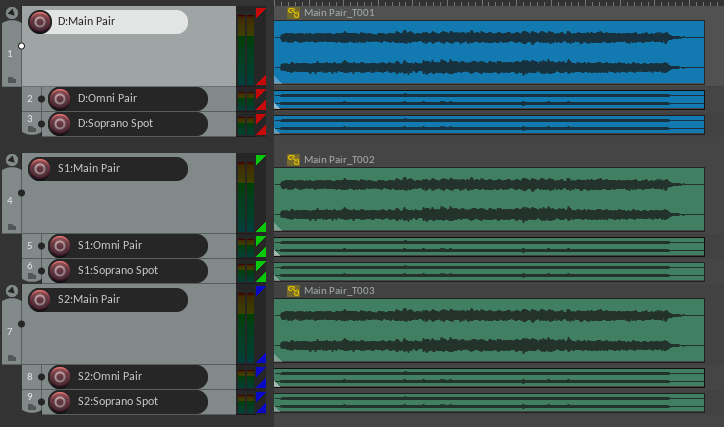
\includegraphics[width=1\linewidth]{user_guide_images/uncollapsed}

\caption{Uncollapsed Track Groups}

\end{figure}

\begin{figure}
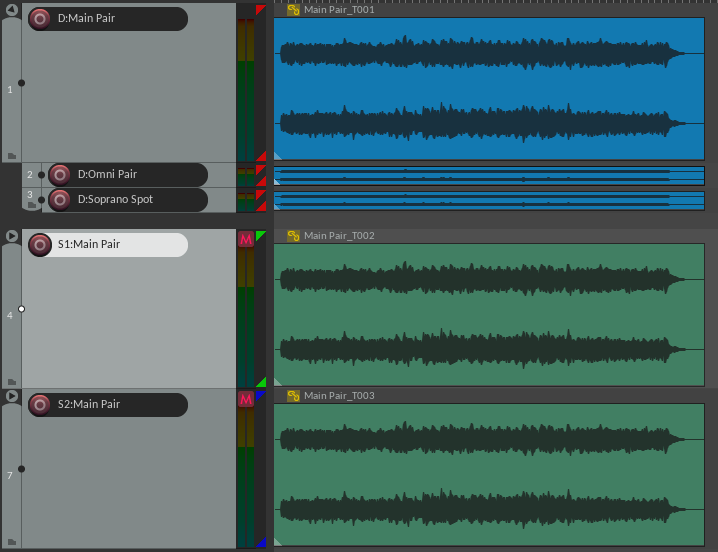
\includegraphics[width=1\linewidth]{user_guide_images/collapsed}

\caption{Collapsed Source Groups}

\end{figure}


\subsection{Peaks Display}

To adjust the visual zoom of wave peaks, use \keys{\ctrl+\arrowkeyup} and
\keys{\ctrl+\arrowkeydown} . This is purely visual and allows for easier editing
of quieter sections.

\subsection{ReaClassical Toolbar}

While I designed ReaClassical to be used efficiently with keyboard shortcuts,
there is a custom S-D editing toolbar for those that prefer it. However I do
highly recommend learning the key strokes as you will find your editing speeds
improve dramatically. The floating toolbar is visible by default on a new
portable install. To open or close, use the \keys{F6} shortcut.
\begin{flushleft}
\begin{figure}[H]
\begin{centering}
\includegraphics[width=0.75\linewidth]{\string"user_guide_images/classical toolbar\string".png}
\par\end{centering} \caption{\label{classical-toolbar-1}ReaClassical custom
toolbar}
\end{figure}
\par\end{flushleft}

From left to right, we have: Destination IN and OUT markers (\keys{1},
\keys{2}), Source IN and OUT markers (\keys{3}, \keys{4}), Delete S-D markers
(\keys{\ctrl+\del}), S-D Edit (\keys{5}), 3-point `Assembly Line' Edit
(\keys{F3}), Insert with Time-stretching (\keys{F4}), Delete With Ripple
(\keys{\backspace}), Delete Leaving Silence (\keys{\ctrl+\backspace}), Set
Destination Tab Project Marker (\keys{\ctrl+alt+1} or \keys{\ctrl+alt+2}), Set
Source Tab Project Marker (\keys{\ctrl+alt+3} or \keys{\ctrl+alt+4}), Delete S-D
Project Markers (\keys{\shift+del}), Copy Destination Material to Source, Move
Destination Material to Source, Reverse S-D Edit (\keys{6}), and finally
ReaClassical Help (\keys{H}).

\subsection{ReaClassical Top Menu}

At the top of the arrange window, you will see a dedicated ReaClassical menu (in
between `Options' and `Extensions'). While not intended to be used as the
primary way of running ReaClassical functions, it is an organized way of
discovering the individual available functions and learning the keyboard
shortcuts.

\subsection{Summary of Track Types in ReaClassical}

While some of these will be covered later in the manual, it is useful to give a
summary of track types you can currently use in ReaClassical. First, we have the
`regular' group or groups of tracks shown in the arrange window. These are where
you record or import takes. You can record-arm tracks and manually select inputs
(if you didn't set during initial setup or via \keys{\ctrl+F9}) here (a reminder
that only locked tracks need only be set on the first group and then \keys{F8}
can be pressed to sync across all groups. Second, we have the mixer tracks
designated via `M:' prefix. These tracks shown only in the mixer are where you
adjust the usual track controls such as names, pan, volume, phase etc. and also
add FX. Their names are synced across the project via \keys{F7} or \keys{F8}.
Third, we have aux busses designated via `@' prefix. You can route mixer tracks
to these to use as a reverb bus etc. Fourth, we have submix busses designated
via `\#' prefix. You can route mixer tracks to these as a way to collect
together microphones from the same orchestral section etc. Fifth, we have a
dedicated room tone track where you can place recorded or generated room tone
(more on this in the mastering section). Sixth, we have the `RCMASTER' bus which
leads directly to the master REAPER bus. Here you can gain stage into the master
bus, add FX etc. Seventh, we have reference tracks which lie outside of the
RCMASTER structure thereby allowing the user to quickly make comparisons with
other imported material via the audition shortcuts. Finally, the master bus
itself where again you can set final levels, add FX etc. As mentioned elsewhere,
try not to delete the mixer tracks or RCMASTER. But, even if you do by accident,
simply run \keys{F7} or \keys{F8} to recreate them depending on your chosen
workflow.

It's important to maintain the prefixes for the special tracks (@, \# and M:)
and to retain the RoomTone, Reference and RCMASTER track names for audio routing
and mixer visibility. However, if you accidentally make improper changes, simply
re-sync via \keys{F7} or \keys{F8} to automatically add back missing prefixes
and correct naming where appropriate. 

\section{Editing}

\subsection{Introduction to Editing Workflows}

Once you have recorded or imported your classical music audio, you are ready to
start editing the raw material! Here we talk about the meat and potatoes of the
classical editing workflows. Workflows---plural---because I have included
different approaches to suit as many tastes as possible within the confines of
the REAPER application. I will explain each in detail after this brief
introduction. As described previously, you have multiple ways of proceeding.
First you can have all your takes lined up in a row horizontally and you place
your source in and out markers, destination in and out markers then press a
keyboard shortcut to achieve your 2-, 3- or 4-point edit. The second way is to
set up your takes vertically and then either use the same marker system to make
your edits or use razor edits (my preferred method when working vertically).
Whichever option you choose, you will then end up in the crossfade editor view
which uses a custom two-lane view with classical crossfade function to make
precise edits really easy in REAPER. I don't often use the fade editor dialog
that comes with REAPER even though I make it appear as part of the function.

\subsection{Marking Edits on your Scores}

This is best done using a physical, photocopied score by the conductor or lead
musician. I advocate for a \textquotedblleft T\textquotedblright{} system where
a large T is inserted into the score at the intended edit point. Either side of
the T stem, and under the crossbar, the outgoing and incoming take numbers are
written. A wavy crossbar indicates some leeway for where the edit point can be
placed. Further notes can be attached underneath the T such as directions for
tightening the gap etc.

\begin{figure}
\begin{centering}
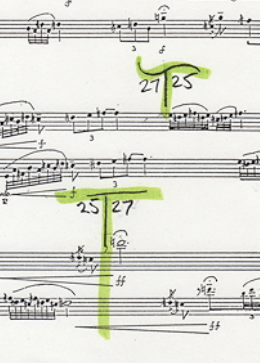
\includegraphics{user_guide_images/score-edits}
\par\end{centering}
\caption{Marking edits on a physical score}

\end{figure}


\subsection{Preparing Takes}

Whether working horizontally or vertically, you can use the Prepare Takes
function. It is intelligent enough to figure out which workflow you are using.
Just press \keys{T} (for `Takes'). Super simple! Every set of items comprising a
take has changed color, is now grouped. In addition, source and destination
groups are linked or (re-linked) for various types of editing. 

\begin{figure}
\includegraphics[width=1\linewidth]{\string"user_guide_images/prepared horizontal\string".png}

\caption{Horizontally Prepared Takes}

\end{figure}

\begin{figure}
\includegraphics[width=1\linewidth]{\string"user_guide_images/prepared vertical\string".png}

\caption{Vertically Prepared Takes}

\end{figure}

If Prepare the `Prepare Takes: Random colors' value is set to 0 in ReaClassical
Preferences \keys{F5} (the default), for horizontal workflows, two shades of
blue are used which also helps show the user where edits happen. For vertical
workflows, the destination group again uses two shades of blue and the source
groups are colored green. In this way they match the colors of the associated
S-D markers. If `Prepare Takes: Random colors' value is set to 1, for
horizontally laid-out takes, each complete take is colored with a different
random color. For vertically laid-out takes, each folder's items are given a
different random color. This way, however you work, it's easy to see where edits
have come from. Prepare Takes can be re-run at any point to re-sync colors and
will preserve any custom colors set via the Colorize function \keys{K}.

In the cases where you might use the function after editing has begun, the
destination group will switch to using alternating colors for items so that you
can easily tell where you have made edits.

\subsection{Auditioning Takes}

For horizontal editing, you could use the usual transport shortcuts (spacebar to
start and stop playback, for example). However, for both horizontal and vertical
editing, it is highly recommended to use the Audition function to quickly solo
only the folder (or track) you are interested in hearing. Just hover the mouse
over the parent for the full mix or a child to solo a spot microphone you want
to hear and press \keys{A} . This includes any @ aux or \# submix track routing
in the signal path. You can easily and quickly create your own custom audition
mix by engaging solo or mute buttons on the mixer, aux and submix tracks (either
with transport stopped or on the fly) and using hover + \keys{A} on the parent
track. You can therefore listen to anything from the full mix down to examining
just the woodwinds submix or a single reverb bus. To audition using a custom
playback rate, use hover + \keys{\shift+A}. The custom playback rate can be set
via \keys{F5}. Note that regular auditioning will automatically reset to the
standard playback rate. 

Don't forget that you can quickly jump to your various source takes using
\keys{\return} and jump to a time within a selected item or crossfaded items
using \keys{\tab} .

\subsection{Source-Destination Editing}

You set your in and out points using special colored labeled markers via
shortcuts \keys{1} and \keys{2} (Destination) and \keys{3} and \keys{4}
(Source). Simply press \keys{5} to make the 2-, 3- or 4-point edit. depending on
how many markers you set. If you attempt to set one of the destination markers
inside of an existing crossfade or within 500ms of a crossfade or item edge, the
function will alert you (pressing OK places the marker anyway). This helps avoid
awkward `sliver' edits that can happen especially if you are zoomed out and
placing markers by ear. You can customize the check range via ReaClassical
Preferences (\keys{F5}). The check range (in milliseconds) is the distance
beyond an item edge, fade or crossfade. For example, setting to 0 would only
check for placement \emph{inside }a fade or crossfade.

You'll also notice that because you prepared the various takes with colors (and
grouping), it is really easy to see which takes compose your final edited
tracks. It's worth pointing out that my S/D and classical crossfade functions
place the crossfade immediately before the entry and exit points of the pasted
audio. The crossfade length and other values can be set on a per-project basis
via ReaClassical Project Preferences (\keys{F5}). In practice this means that if
you visually set a marker (or edit cursor in the case of the classical crossfade
function) immediately before a transient, said transient will sound
post-crossfade which is what we generally desire. Often, given this important
detail, I don't even need to visit the crossfade editor view.

When using a vertical workflow, make sure you have the source folder selected
before you create the source IN and OUT markers. You can do so by clicking on
the item at the locations you want to set the markers. This adds the folder
number as a prefix to the source marker labels. The various functions will then
use this label to know which folder to copy from. This is really useful if you
undo the edit in order to tweak the markers by dragging them. It doesn't matter
if you then select other folders/tracks. In the event you use two different
folders for the source IN and OUT markers, the functions will prefer the source
IN label.

The downside to this workflow when using a vertical approach is that the source
and destination markers can get in each other's way visually if the takes aren't
somewhat staggered, however the process still works as expected. See below for a
razor editing alternative.

\emph{Optional: If you are worried about accidentally moving markers and items
during precise S-D or assembly editing, engage the padlock icon in the top-left
of the ReaClassical window. By default with the latest ReaClassical project
template, it should prevent manual left/right item movement and marker dragging
(while still allowing for S-D editing with ripple). Even though you can't move
S-D markers by dragging with this lock mode engaged, you can still use the
shortcuts }\keys{1}, \keys{2}, \keys{3} and \keys{4}\emph{ to change marker
location. Just remember to disengage lock mode when you enter the fade editor or
else you won't be able to move the items of the crossfade!}

\subsubsection{\label{subsec:Multi-Project-Tab-S-D}Multi-Project Tab S-D
Editing}

If you'd like to S-D edit between various open project tabs you can set both the
source and destination `project' markers via \keys{\ctrl+\Alt+1} (or
\keys{\ctrl+\Alt+2}) for destination and \keys{\ctrl+\Alt+3} (or
\keys{\ctrl+\Alt+4}) for source (essentially the same numbers associated with
regular S-D markers). The markers can exist anywhere on the tab's timeline but
perhaps the very beginning or end would be good to keep them out of the way. The
S-D editing itself then works just as for a single tab other than any source
markers that are set are not deleted to aid quickly undoing in the destination
tab and being ready to reapply the edit. The only rule when using S-D project
markers is to ensure that source or destination markers should be paired with
the corresponding source or destination project marker. This workflow would, for
example, allow you to have multiple project tabs (perhaps one for each symphony
movement plus a final `destination' tab), allowing for both internal editing per
tab but after setting the S-D project markers compiling the final edit in the
`destination' tab. To delete all the S-D project markers press
\keys{\shift+\del}. Also, in multi-tab S-D editing, when regular markers are
placed, any other existing versions in other tabs are automatically deleted to
ensure that only one version of the marker exists at a time across all open
project tabs.

\begin{figure}
\begin{centering}
\includegraphics[scale=0.5]{\string"user_guide_images/S-D markers\string".png}
\par\end{centering}
\caption{Source-Destination Markers}

\end{figure}


\subsubsection{4-Point Editing}

For this operation, set all four markers using \keys{1} , \keys{2} , \keys{3}
and \keys{4} . Make the edit with \keys{5} . This is the most useful edit when
dealing with classical music or other acoustic music performed without a
metronome.

\subsubsection{3-Point Editing}

For this operation, set any combination of three markers. Again, make the edit
with \keys{5} . The missing marker is placed according to the distance set by
the existing complete pair. 

\subsubsection{2-Point Editing}

For this operation, there are two possibilities: 1) Set one source marker and
one destination marker. Make the edit with \keys{5} . Any missing IN markers are
set to the beginning of the timeline and any missing OUT markers are set to the
end of the source or destination material. 2) Set both source markers and no
destination markers. Make the edit with \keys{5} . Here, the destination markers
are set at the exact same positions on the timeline as the source markers.
Obviously this operation is only useful in a vertical editing workflow when you
can select source material from a different track group. The usefulness of this
second option is further reduced if the takes are not vertically aligned and not
virtually identical in tempo. On the other hand, it could be an incredibly quick
method for editing takes of a hybrid classical piece that is performed to a
click track or other recorded steady beat.

\subsection{Other SD Functions}

\subsubsection{Insert with Time-Stretching}

Using the ReaClassical\_Insert with time-stretching function \keys{F4} , you can
complete a 4-point edit where the material between the source markers is
time-stretched to fit the length of time between the destination markers. This
is really useful when the source material has to fit the destination span
exactly, for example when working with visual cues. The time-stretch algorithm
used will be the one set in REAPER project settings. When there are multiple
items in between the source markers, the function will glue the items together
before time-stretching. Note that this function can also be used in multi-tab
S-D editing mode (see above).

\subsubsection{Assembly Line Editing}

Sometimes you don't necessarily have a best overall take and it is desirable to
build the perfect performance linearly, section by section, measure by measure.
In this case, set the destination IN marker with \keys{1} and set both source
markers using \keys{3} and \keys{4}. Press the \keys{F3} shortcut. A 3-point
insert operation will occur and the destination IN marker will jump to the end
of the pasted item, ready for the next edit. This means that in order to compile
further sections, you now only need set the source markers. If you accidentally
move the location of the destination IN marker in the middle of assembly line
editing, the function will let you know and offer to move the marker back to the
right edge of the latest item in the edit. This will even allow you to do some
regular 3- or 4-point editing earlier in the sequence before continuing with the
assembly line edits. Just place the destination IN marker anywhere in the
project and answer `No' when the message box appears. Note that this function
can also be used in multi-tab S-D editing mode (see above).

\subsubsection{Delete / Delete with Ripple}

While perhaps not used as often as 3- and 4-point edits, I have created two
functions for deletion of material. Delete \& Ripple \keys{\backspace}
(backspace) will delete the material between source IN and OUT markers and
ripple material to the right backwards with a short crossfade. Delete Leaving
Silence \keys{\ctrl+\backspace} will also delete but maintain the silence
without rippling backwards.

\subsubsection{Copy/Move Destination Material to Source}

Run either the copy or move version of the function from the ReaClassical
toolbar (no need to ensure the first track is selected) and the function will
copy or move all items and edits from the destination group directly below to a
newly created source group with "Eastern" Blue color for identification
purposes. This allows for saving versions of finished edits either via iteration
(\textit{copying} so you can continue to make further edits) or fresh
(\textit{moving} so you can compile an alternate version of a "best" take from
scratch). These different edits can then be easily auditioned via the \keys{A}
shortcut. This is similar to a Pyramix-style iterative editing method while
still maintaining the destination group as the uppermost group.

\subsubsection{Reverse S-D Edit}

Place your destination markers using \keys{1} and \keys{2}, then set a source IN
marker with \keys{3}. Pressing \keys{6} will copy or move the material between
the destination IN and OUT markers to the selected source group, as determined
by the \keys{3} shortcut. Upon execution, you will be prompted to choose whether
to copy or move the material. This function operates similarly to the
\textbf{Copy/Move Destination Material to Source} functions but allows for
precise selection using S-D markers. It is particularly useful for editing a
single section like a \textit{da capo}, where you may want to construct an edit
using material from the first run-through without having to scroll back and
forth along the timeline. For example:

\begin{itemize}
    \item To use material from the first run, copy it to an existing empty
    \textit{placeholder} source group using \keys{6} (answering ``No'' when
    prompted to delete the destination material), then manually position it
    under the second run.
    \item If the da capo material serves as a strong foundation, you can leave
    it in place on the destination group. Alternatively, you can move the da
    capo material to a second empty source group using \keys{6}, selecting
    ``Yes'' when prompted to delete the destination material.
\end{itemize}

\subsubsection{Add S-D Markers to Edges of Item(s) or Time Selection}

Used in combination with Delete / Delete with Ripple (\keys{\ctrl+\backspace} /
\keys{\backspace}), you can quickly set both source markers to the edges of one
or more selected items on a parent track or time selection via \keys{F12}. This
is a time-saver when dealing with potential `sliver' edits i.e. small unneeded
leftover edits as a result of multiple rounds of zoomed-out S-D editing. Note
that the built-in checks when manually placing destination markers should go
some way to alleviating this issue which can easily go unnoticed in other
classical music DAWs. Likewise you can use \keys{\ctrl+F12} to set destination
markers (selected items must be in the destination folder). Note that if using
time selection for placing source markers, as for S-D marker placement via
\keys{3} or \keys{4}, make sure you first have the desired source folder track
selected before pressing the shortcut (a good way to do this is to first click
on the item involved). You may prefer to set both source and destination markers
this way over the more traditional number key shortcuts acting as a sort of
hybrid between S-D and razor editing. Also note that if both selected items and
a time selection exist, the time selection takes precedence.

\subsubsection{Move / Zoom to S-D markers}

To move to any existing S-D markers use \keys{\ctrl+1}, \keys{2}, \keys{3} or
\keys{4}. To zoom to any of the S-D markers for more fine-grained placement, use
\keys{\Alt+1}, \keys{2}, \keys{3} or \keys{4}. If you have multi-tab S-D editing
set up (see \ref{subsec:Multi-Project-Tab-S-D}), these shortcuts will also
automatically move focus to the correct project tab. 

\subsubsection{Delete S-D markers}

To delete all regular S-D markers, press \keys{\ctrl+\del}.

\subsection{Floating Destination Group}

The floating destination group feature enhances vertical workflow efficiency by
dynamically positioning the destination group just above the selected source
group. This reduces unnecessary vertical scrolling when setting IN and OUT
markers for destination and source groups that are far apart in the project.
Additionally, this feature is fully compatible with mouse hover S-D editing.

To enable the floating destination group, open ReaClassical Project Preferences
(\keys{F5}) and set the corresponding value to ``1''.

For example, with floating destination enabled, place a source IN marker (via
\keys{3}) on any source group. The destination group will reposition itself just
above the selected source group. Add the remaining S-D markers as required.
Perform any S-D edits via \keys{5}, \keys{F4}, or \keys{F3}. Select another
source parent and place another marker (\keys{3}). The destination group will
continue adjusting dynamically. 

To disable floating mode, re-open ReaClassical Project Preferences and set
``Floating Destination Group'' back to ``0''.

It is worth noting that if the destination group moves above a source group, the
source marker track number correctly updates to reflect the new order. 

\subsection{Razor Editing}

Because of the potential for visual overlap of markers, I much prefer the REAPER
razor edit functionality for vertical take work. It works a lot like the process
shown in this Pyramix \href{https://www.youtube.com/watch?v=wQXwnvITQCQ}{video}.

While Pyramix also has additional source-destination marker workflows, I
couldn't help but feel that for professional ensembles that manage a high degree
of tempo regularity between takes, this method can be extremely efficient. This
isn't the document to introduce REAPER razor edits as there are plenty of
resources online if you do a simple search. Here we are only concerning
ourselves with creation of the razor area across all our pairs and spot mics
(REAPER's default shortcut is the rather uninspiring Alt+Right drag).
Thankfully, it can become the default editing mode by selecting the razor edit
mode on the main toolbar and left-click dragging. 

\begin{figure}
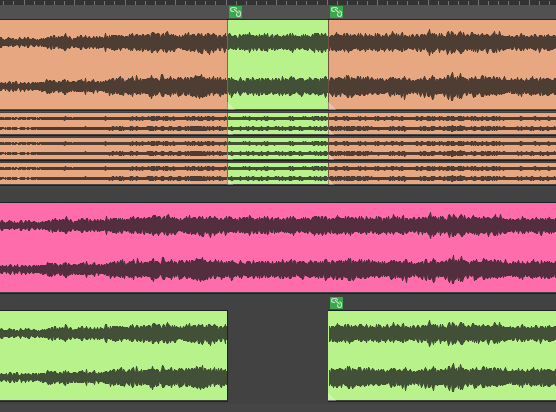
\includegraphics[width=1\linewidth]{user_guide_images/razor}

\caption{Razor Editing}

\end{figure}


\subsection{Crossfade Editor}

Now that you've made your precise edits using S/D workflow or razor editing (no
worries if it's a bit rough!), it's time to check things through with the help
of the crossfade editor view.

While REAPER includes an excellent crossfade editor, it does not reach the same
levels as the ones in specialist classical DAWs such as Sequoia and Pyramix.
This is mainly due to the inability to see the continued waveforms of the items
beyond the crossfade they enter and likewise the previous waveforms of the items
that exit the crossfade. The ability to visually align transients and then
position the crossfade just before it is absolutely critical (and fun when you
have the tools to do it!). So, beyond the standard REAPER crossfade editor what
have I provided? Select the right-hand item of a fade (or hover over the item if
`Add S-D Markers at Mouse Hover' is set to 1 in ReaClassical Project Preferences
\keys{F5}), press \keys{F} and you are moved into crossfade editor mode. Here,
the first track is given full vertical zoom, the two-lanes for overlapping items
is enabled, colored red and green, and the fade editor toolbox appears (I
personally position it to hover over the middle of my mixer. Note also that you
are automatically centered on the crossfade and can use the mouse wheel to zoom
in and out. Press \keys{F} again and you exit that mode. If for some reason you
accidentally close just the fade toolbox, either open again using action in the
action list or, better still, simply close and re-open the fade editor using
\keys{F} .

So, now you are in the crossfade editor mode, ensuring one or both items are
selected, hover your mouse over a blank area and press \keys{Z} to automatically
mirror extend the waveform view of each item. Essentially, it increases the
overlap so you can spot and align the transient you want. My own preferred
method of getting the perfect crossfade is to locate the transient I want on the
red left item, place the edit cursor just before it, then drag my green right
item so that the two transients align. Then I press \keys{X} (classical
crossfade) and I'm done! The crossfade happens at the location of the edit
cursor (well, just before it as explained above). 

I love this method so much that I don't miss Sequoia or Pyramix any more. Here
it is in ordered list form:
\begin{enumerate}
\item Increase overlap (by hovering mouse either in a blank area or over one of
the items and pressing \keys{Z} shortcut to mirror extend the item edges)
\item Find transient in red left item that you want be edit point
\item Place edit cursor just before it
\item Drag green right item to align transients (this automatically ripples all
items, markers and regions)
\item Press \keys{X} (classical crossfade)
\end{enumerate}
\begin{figure}
\includegraphics[width=1\linewidth]{\string"user_guide_images/xfade window\string".png}

\caption{Crossfade Editor View}

\end{figure}

In reality, this process can be just a few seconds to achieve the perfect edit.
In the unlikely event you need to undo, either use the standard \keys{\ctrl+Z}
combination or simply extend the overlapping item edges again then create a new
classical crossfade.

While you could use the auditioning tools in the dialog, I have created
something I find quicker and more useful. While the two items involved in the
crossfade are selected, try the following:
\begin{enumerate}
\item Hover over left item / press \keys{A} to solo audition the left item from
mouse cursor to end of item
\item Hover over right item / press \keys{A} to solo audition the right item
from start of item to mouse cursor
\item Hover in blank space on left item side / press \keys{A} to solo audition
the crossfade from mouse cursor to mirrored position on the other side of the
crossfade
\item Hover in blank space on right item side / press \keys{A} to solo audition
the crossfade from mirrored position other side to the mouse cursor.
\end{enumerate}
\begin{figure}
\includegraphics[width=1\linewidth]{\string"user_guide_images/xfade auditioning\string".png}

\caption{Crossfade Auditioning Tools}

\end{figure}

As you'll see, the playback stops using a special marker with {*}!1016{*} as the
label which is executed as a stop command. It is deleted automatically after
playback ends. If you try to run the function another time before it has
finished, just select new instance if you get a pop-up box. You can stack
instances and on completion of the latest run, all instances are removed. Better
to experience than describe but it works really well. You'll also see that the
edit cursor returns to the middle of the crossfade to aid in mouse scroll
zooming keeping the crossfade centered. The mirrored position takes into
consideration the overlap of the items so you can have a complicated set of
fades and still get an exact mirrored stopping point.

You can shuttle between crossfades using the \keys{Q} and \keys{W} shortcuts. Do
\textbf{NOT} use the built-in Previous Next buttons on the standard fade dialog
box! However, there is still a benefit of having the fade editor dialog in view.
You can also tweak the fade using the knobs if you prefer. Center, Start, End
and Length knobs are particularly useful here to maintain symmetry. Be aware
that the Contents knobs will not ripple markers (but with the introduction of
the Create CD Markers, I highly recommend not bothering to create any markers at
this point).

\subsection{Other Editing Tips}

In my key map, I include all sorts of useful shortcuts to use during editing. As
mentioned above, in vertical editing workflows, the Audition function \keys{A}
is brilliant for listening to various takes before applying a razor or S/D edit.
I can shuttle between items with \keys{Q} and \keys{W} (the same keys perform a
more advanced role when in crossfade editor mode), shuttle between markers with
\keys{,} and \keys{.} (the same keys with \keys{<} and \keys{>} on them on my UK
keyboard), \keys{S} for splitting a long recorded session into takes, \keys{`}
(back tick) and \keys{\ctrl+`} for zooming out to the whole project both
horizontally and vertically etc. There are plenty more for the mastering end of
things so I encourage you to explore.

It is worth noting that all regular markers and regions are ripple edited
appropriately when using my source-destination editing functions and crossfade
editor. I also introduced the ReaClassical\_Lock Toggle function \keys{K} which
temporarily locks all source groups and engages ripple-all-tracks mode to enable
you to drag destination items and simultaneously ripple markers and regions in
the regular arrange view. This allows vertical source groups to retain their
independence yet still give ripple-all-tracks behavior which is useful for
destination album track spacing etc. However, I consider this function
deprecated given I strongly feel that the Create CD Markers function is now the
ultimate way to deal with CD tracks/markers.

\section{Mixing}

\subsection{FX Plugins}

ReaClassical is shipped with various mastering-grade JSFX plugins to cover
typical needs although obviously REAPER allows for any 3rd party plugins. For a
list of recommended free plugins see Appendix C. In ReaClassical, you should add
plugins to the dedicated mixer tracks. 

\subsection{Aux \& Submix}

Users have the ability to create aux and/or submix tracks that stay visible (and
stay after the mixer tracks). To set up, simply create a single folder via
Horizontal Workflow \keys{F7} and/or Vertical Workflow \keys{F8} then create as
many aux/submix tracks after the mixer tracks as you like via \keys{\#}. It is
important to keep the @ or \# at the beginning of the track but you can add any
name you'd like e.g. `@hall-verb', `\#strings'. To route, click-drag from a
mixer track's routing stripes to the desired @ or \# track. When using any of
the ReaClassical functions such as auditioning, these tracks will remain
visible.

For \# submix tracks, simply add a hyphen (-) at the end of desired track names
in the mixer tracks and sync via \keys{F7} or \keys{F8}. Now those related mixer
tracks will not route directly to RCMASTER. As an example, say mixer tracks 3-6
are all string section microphones and you'd like to sum them all to a string
submix track called `\#strings'. Just add a hyphen to the end of the names for
mixer tracks 3-6, sync and then create the routing to \#strings via
click-dragging from the routing stripes. This routing is maintained during
\keys{F7} or \keys{F8} syncs.

\subsection{Roomtone}

In a live concert recording that contains audience noise in between movements
and applause at the end of a complete piece, it is often desirable to give the
impression of a clean recording with no audience present. Recorded or generated
room tone then becomes very important as an alternative to audio fading to
complete digital silence which destroys the illusion of listening back to a live
concert. ReaClassical includes a dedicated room tone track for this purpose.
This way, the auditioning tool will keep the track displayed in both track and
mixer panels. Add via \keys{\#}. Once added, you can add clean recorded noise
captured before or after the concert or generate endless roomtone the length of
your project from a very small portion of clean silence from the concert itself
(hint: try using a white noise generator into a convolver such as ReaVerb that
uses a few seconds of clean room tone as the impulse!). As of ReaClassical
24.12, the Create CD Markers function automatically generates precise volume
automation at the track level to seamlessly fade in and out of room tone! See
the mastering section for more details. Please not that there is a limit of one
reference track per project.

\subsection{Reference Track}

Add a reference track via \keys{\#} to allow for importing a commercial album
track or similar to help achieve the desired loudness levels, EQing etc for your
own material. The reference track is deliberately placed outside of the RCMASTER
structure and can therefore be quickly auditioned independent of any effects you
have on the mixer and RCMASTER tracks.

\subsection{Maintaining/Breaking Connections to RCMASTER}

When adding special tracks via \keys{\#}, set \textquotedbl Maintain Mixer =>
RCMASTER\textquotedbl{} to 0 to add a hyphen (-) to the end of every mixer
(``M:'') track thereby removing the direct connection to RCMASTER allowing for
all sorts of custom routing via submixes etc. By default, the final option is
always set to 1 to maintain the current routing.

\section{Mastering}

Mastering in ReaClassical is game-changing. Many features described here are not
available in any other classical DAW. I hope that the `ReaClassical' way saves
you much time and helps you look forward to the mastering phase of the project.
While automatic DDP generation, automatic room tone function, and professional
album reports are the main features here, you will probably find the
revolutionary automation mode is an extremely efficient way to add static mixer
scenes across your production as well enjoying the ability to quickly reorder
album tracks via a simple keyboard shortcuts.

\subsection{Mastering Mode}

Change to mastering mode via the shortcut \keys{\ctrl+M}. In addition to making
the mixer tracks, busses and RCMASTER available in the arrange window for
setting static mixer scenes via envelope points, it also serves to de-clutter by
hiding any source group audio. The hide and show child tracks shortcuts still
work on the destination folder but in mastering mode also works on automation
lanes. Simply select the relevant track connected to the lane and use the usual
\keys{E} and \keys{D} keys to hide and show automation lanes. Look out for more
`mastering' mode features in the future.

\begin{figure}
\includegraphics[width=1\linewidth]{\string"user_guide_images/mastering mode\string".png}

\caption{Mastering Mode}

\end{figure}


\subsection{Automation}

Given ReaClassical is built on top of REAPER, it allows for same high-quality
automation workflow with a ReaClassical twist. Beyond the following workflow
descriptions, it is recommended to read the relevant REAPER manual section as
there are far more features than can be described here. For example, you can add
static mixer and FX `scenes' to automation lanes (very useful for quickly
setting up different settings for the various pieces on an album) . It makes
most sense to leave any automation work until the destination group editing is
largely complete. Start automation mode via \keys{\ctrl+I}. Mastering mode will
be enabled automatically as needed. All the envelope buttons will turn blue
(`latched preview') and you will see a message box with instructions. Simply set
any desired mixer controls or parameters in an open FX window) on one or more
tracks and press \keys{I} to enter the values as points on the automation lanes
at the edit cursor position or, if one exists, within the time selection.
Continue to add, edit or audition and once completed, exit `automation' mode via
\keys{\ctrl+I}. The envelope buttons will then turn green (`read' mode).
Hopefully this `ReaClassical' way can make things faster and easier at the same
time. Once multiple static mixes have been set up, you can then, of course, use
more detailed automation via the pencil tool or riding the fader to, for
example, temporarily bring up spot microphones. 

In addition, there are also take envelopes that you can access via
right-clicking on an item and going to \menu{Take > Take Volume Envelope}. This
is incredibly useful for transparently reducing very short stray peaks versus
using a limiter. Simply create a selection over the problematic area by
left-click-dragging and then \keys{\ctrl+\shift} and drag up or down to just
affect that portion of the envelope without needing to add in individual points.
It's such a time-saver! The benefit here is that you can also see how the item
waveform is affected in real time.

If you want to exit both automation and mastering modes, press \keys{\ctrl+M}.

\subsection{Repositioning Tracks in an Album}

There are two functions which help with reordering or repositioning tracks.
First, and perhaps most useful for producing a classical album, is if you decide
that you need to reorder one or tracks. Simply select the track you want to move
and press either \keys{\ctrl+\arrowkeyleft}or \keys{\ctrl+\arrowkeyright} to
switch with the track immediately to the left or right. Note that gaps are
preserved too. 

The other situation is when you want to start with uniform gaps between a series
of short separate pieces. Use the \keys{\ctrl+Y} shortcut and enter a value in
seconds. Your pieces are then automatically spaced and items crossfaded are left
intact.

\subsection{Loudness}

In terms of loudness, I personally aim for about -18 LUFS Integrated for my
classical albums though it can be as high as -16 LUFS and as low as -20 LUFS.
The new loudness JSFX meter in REAPER along with the normalization of loudness
and true-peak limiting in the render dialog are priceless. It's another reason I
couldn't go back to the big classical DAWs at this point.

\subsection{Metadata}

To quickly remove all the take names on the destination parent track, run
\keys{\ctrl+T}. Track titles are then added to the individual items on the
destination parent track by double-clicking on the item or selecting and
pressing \keys{F2}. Note that only items that start tracks should be named. 

The rest of the metadata is then added via the Create CD Markers function
\keys{Y}. You can add UPC/EAN and ISRC numbers as desired followed by album
title, performer, composer and genre. On later runs of the function, you can
choose to automatically re-use existing values which can save even more time
when making last-minute S-D edits, altering album spacing, switching album track
order, or renaming a CD track start.

\begin{figure}
\begin{centering}
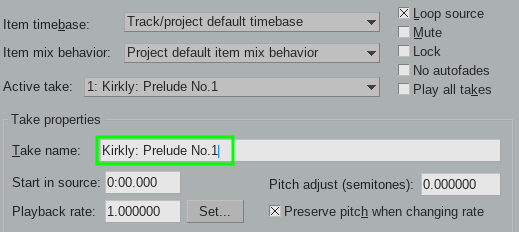
\includegraphics[scale=0.75]{user_guide_images/takename}
\par\end{centering}
\caption{Adding Track names}

\end{figure}


\subsection{Creating DDP filesets}

I have introduced a workflow to automatically add the CD/DDP markers, regions
and room tone automation via \keys{Y} (track and region names are pulled from
item take names, markers/regions auto-snap to CD frames, initial 2-second
pre-gap, silent roll out and album metadata also added!) . It is \textquoteleft
smart\textquoteright{} in the sense that if there's no take name, no marker or
region will be created. In other words, press \keys{F2} with an item selected to
enter track names where markers/regions need to be created. It's perfect for
classical releases where a crossfaded item is likely an internal
source-destination edit versus a new track. For CD tracks that you want to have
a visual CD player countdown, simply start the item name with an exclamation
(!). Preferences such as CD marker offset, pre-gap length and album lead-out can
be set via ReaClassical Project Preferences \keys{F5} . So it's now very quick
to export a DDP set!

\noindent\fbox{\begin{minipage}[t]{1\columnwidth - 2\fboxsep - 2\fboxrule}%
If working in horizontal workflow, ensure that there is over a minute's worth of
empty timeline between the end of the proposed album and any other source
material. Instead, you can also choose to drag any source material to a new group by
first creating an empty duplicate folder via \keys{\textbackslash}.%
	\end{minipage}}

Further, you can add audio to the initial pre-gap (an `easter egg' track) by not
giving the first item (or crossfaded items) a take name. The function will
assume that this is supposed to be hidden and generate the initial pre-gap
length accordingly. 

If a room tone track is present in the project, the function will also generate
precise track-level volume automation that creates perfectly-matching fades at
points where items fade into and out of silence on the first destination track.
In other words, slicing and dicing room tone audio to fill in digital silence is
no longer necessary in ReaClassical!

For more information read the description of the DDP function in appendix A.

\subsection{Creating CUE Files}

A CUE file is automatically generated as part of the Create CD Markers function
(\keys{Y}). You can change the production year of the project as well as the CUE
audio format in ReaClassical Project Preferences. The high-resolution audio
portion can be generated separately in the render dialog via the preset. The
naming defaults to that set by the CUE file which is the project filename
followed by the audio extension set via \keys{F5}.

\subsection{BIN+CUE set}

Create a BIN/CUE pair (either select `regions define tracks\textquoteright{} and
render the whole project or select `use only \# markers' and render by time
selection if you don't want the first pre-gap as actual silence at the start of
track 1). 

\subsection{Album Reports}

When using the \keys{Y} shortcut, ReaClassical also generates both a plain text
and HTML album report in the project folder including details such as pre-gaps,
track title, start time, track length, UPC/EAN and ISRC (if present), total
running time etc. This is a fantastic and automatic way to send information to
clients or a duplication/replication factory.

\begin{figure}
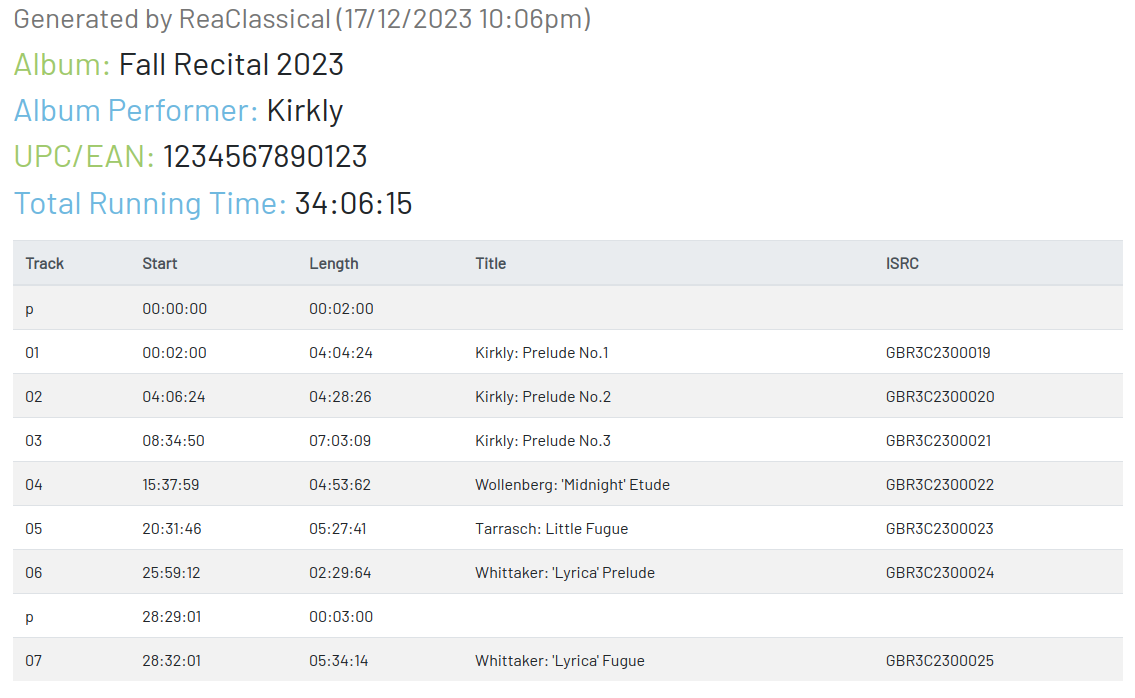
\includegraphics[width=1\linewidth]{user_guide_images/html_album_report}

\caption{An example of an automatically generated HTML album report}

\end{figure}


\section{Rendering}

\subsection{Presets}

ReaClassical includes various rendering presets to make rendering extremely
quick and easy. In the Render dialog \keys{R}, click on the presets button then
`All Settings'. The preset names are self-explanatory. The first four entries
are for exporting a whole album as a single audio file. The remaining use the
automatically created regions after using the Create CD Markers function
\keys{Y} to create automatically named folders of audio files, one per CD track.
After selecting a preset, you should feel free to change any render settings and
perhaps save as a new preset for future use. By default, the presets use the
built-in REAPER standard triangular dither.

\begin{figure}
\begin{centering}
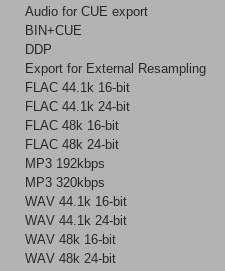
\includegraphics[scale=0.75]{user_guide_images/render_presets}
\par\end{centering}
\caption{ReaClassical Render Presets}

\end{figure}


\subsection{Samplerate}

Now that r8brain free has been introduced as the best quality resampler
available in REAPER (I highly recommend double-checking that it is selected when
resampling at render time) I feel I can do everything, including DDP creation,
without leaving my favorite DAW. However, generating a CUE file via the Create
CD Markers function is still useful for all sorts of things and I often create
FLAC + CUE for album playback in my media player or WAV + CUE to easily burn a
CD at home.

\subsection{Dither}

Use either the built-in REAPER dither options or RCDither as the last plugin on
the master chain. If using RCDither or any other 3rd-party dither be sure to
keep the master fader at unity and disable all REAPER dither checkboxes.

\subsection{Loudness \& Limiting}

REAPER has a fantastic rendering feature which allows the user to set a desired
loudness and peak / true peak setting. For quick exports that need to meet
certain targets (i.e. streaming) this makes things extremely efficient and is
very transparent when not set to extreme values.

\subsection{Dry-run Rendering}

Another REAPER feature that is outstanding is the dry-run render function which
allows for very quick offline loudness and peak checks and much faster than
using REAPER's included realtime loudness meter. It is therefore extremely easy
to set up compressors, limiters etc in the project and make small adjustments
based on the dry-run values and maintain complete control over the process. 

\subsection{Other Rendering Tips}

Not necessarily obvious to new REAPER users are the special =START and =END
markers (make your markers in the usual way and label them accordingly) that
constrain the length of the project. Rather than rely on extended silence at the
end of items or time selections, the =END marker is a great way to ensure you
have the exact amount of lead-out you want at the end of the disc. Positioning
both special markers is great way to generate files for multi-disc releases
without having to rely on multiple projects.

You will hopefully notice I have included various shortcuts for manually
creating regions (single or multiple) from items and time selection (great for
quickly generating demo snippets). Also worth noting is that you can still do
some (or all!) of your source-destination editing with your track markers in
place as the S/D markers have IDs far higher than any classical CD would have
and are automatically deleted after a successful edit. As long as you have your
ripple-per-track mode engaged, all your existing marker placements and carefully
crafted edits will remain intact. But, again, don't manually create CD markers
at this point as I include a very powerful tool to make light work of that side
of mastering.

\section{Project Management}

\subsection{Statistics}

For a complete set of statistics on the ReaClassical project, either for your
own information or to assist with billing a client, go to \menu{ReaClassical >
Utilities > Show Statistics} or use the shortcut \keys{F1}. For example, you might have a billing system that
charges clients based on number of source-destination edits, or mixing/mastering
based on the final length of the album. Information includes: final album
length, number of CD markers, project age, total project length, total length of
source material, total number of items, number of track folders, number of
tracks per group, number of ``special'' tracks, number of regions, number of
destination S-D edits, number of destination item splits, FX count and number of
automation lanes.

\subsection{Typing Notes}

Document your takes either using the built-in REAPER project notes or SWS Notes
\keys{N} (for `Notes') which can be attached to items, tracks, markers etc. I
personally prefer item notes on the main microphone pair. It's a very useful
tool to have docked at the bottom of the screen.

\subsection{Folder Structure}

ReaClassical defaults to placing media and exports into appropriately subfolders
making project file navigation easier. Also, ReaClassical defaults to separate
folders for automatic backups and auto-saves. These settings are subject to
change and can be modified by going to the REAPER preferences \keys{O} (for
`Options').

\subsection{Automatic Backups}

REAPER allows for powerful and complex backup routines. As referenced above,
ReaClassical defaults to 10 time-stamped backups and 10 auto-saves every 15
minutes when not recording. Feel free to modify for your own way of working
including switching to backups and auto saves for a number of unique days.

\subsection{Cleaning}

If in doubt, keep everything! Otherwise, the \menu{File > Clean current project
directory} is an excellent way to reduce the size of your projects. Note that
when assigning a session name via the Take Counter Window, currently the above
REAPER menu item doesn't search recursively. In a way, this reduces the chances
of accidentally deleting precious takes. You can always manually delete but,
from experience, it is \emph{much} better to simply keep everything.

\subsection{Archiving}

There are various ways to archive classical music projects. First, you can
access the Project Bay by \keys{\ctrl+B} shortcut. You can then ensure that all
media used in the project is contained within the project folder itself. If not,
you can select as many as necessary, right click and move/copy into the project
folder. After this, you can simply compress the folder as a zip and store on an
external drive. A further step to guaranteeing ability to open in the future is
to freeze tracks so that plugin effects are baked in (with ability to unfreeze
later if possible). Alternatively you can save a copy of the project via
\menu{File > Save project as...} \emph{,} converting to a format like FLAC and
trimming the media as you wish. Finally, one to look out for in the future is
\href{https://forum.cockos.com/showthread.php?t=280150}{Project Archiver}.
However, I don't believe it is quite ready for prime-time yet and recommend
using one of the other methods for now.\pagebreak{}

\part{End Matter}

\section{Thanks}
\noindent\begin{flushleft} I am appreciative of the collective contributions of
the REAPER community with regards the early source-destination actions (Pelleke,
in particular), MPL, X-Raym, BirdBird, RCJacH, Sai'ke, Meo-Ada Mespotine,
cfillion and many more. Finally, many thanks to Justin and Schwa for such an
amazingly versatile DAW. \par\end{flushleft}

\section{Closing Thoughts}
\noindent\begin{flushleft} I hope you enjoy the ability to do serious classical
editing with ReaClassical on REAPER and that my efforts go some way to making
things better, easier and more efficient. Remember that if you find any oddities
with the functions or have a bright idea for something new and shiny, please add
your thoughts to the
\href{https://forum.cockos.com/showthread.php?t=265145}{dedicated thread} on the
forums and/or create an issue or start a discussion on my GitHub repository
located at
\href{https://github.com/chmaha/ReaClassical}{https://github.com/chmaha/ReaClassical}.
\par\end{flushleft}

\pagebreak{}

\appendix

\part{Appendices}

\section{Description of ReaClassical Functions}

\emph{Preliminary Note: }These proceed in a quasi-workflow order. I include the
default shortcut keys if using my portable install or resource folder base. You
can also use the custom toolbar via the mouse. 

\textbf{Create/Sync Horizontal Workflow }\keys{F7}

\emph{Description: }The way to create a horizontal workflow with a single folder
group with as many tracks as you need. It can also be used with an single
existing folder group to re-sync track names and re-build project routing.

\emph{Notes: }Use on a completely empty project. I would use this if you are
planning to use a horizontal approach to source-destination editing (i.e. the
various takes are laid out from left to right) or if you want a quick way to set
up a mixing/mastering track set with a single take. The function automatically
sets up the tracks for group media and razor-editing along with dedicated mixer
tracks. These mixer tracks should be used for all track settings (names, volume,
pan, polarity, sends and FX).

\textbf{Create/Sync Vertical Workflow }\keys{F8}

\emph{Description: }A multi-use function to 1) set up a vertical workflow with
destination and source groups with as many tracks as you need, 2) to create
source groups from an existing destination folder group (for example, created
with \keys{F7} shortcut) and, for in the middle of editing, 3) to (re)create
project routing and sync track-naming, record inputs and lock states. Note that
for 3), all folders should contain the same number of tracks.

\emph{Notes: }For all track settings (names, volume, pan, polarity, sends and
FX) you should use the dedicated mixer tracks.

\textbf{Explode multi-channel item }\keys{F10}

\emph{Description:} Explode multi-channel item(s) to either all mono or
stereo-interleaved + mono

\emph{Notes:} Import your multi-channel media using a single regular track (for
a horizontal workflow) or multiple regular tracks (for a vertical workflow).
Then, simply press \keys{F10} (no need to select the items). Answer yes to the
prompt that appears if the first two channels should be treated as stereo
interleaved (i.e. they represent your main pair). Depending on the choice made,
the number of tracks in the resulting folder(s) will adjust accordingly. Then
you are given the opportunity to name your tracks. Obviously if you decide to
move to a vertical workflow after exploding using a single track, you can always
use \keys{F8} to create your source folders then drag the media to where you
want them. If you need to bring in new takes after editing has started, simply
use the function on an empty project tab then copy or cut them into the original
project tab into the desired folder on the timeline.

\textbf{Add special track(s) }\keys{\#}

\emph{Description: }Adds one or more special tracks (aux, submix, roomtone,
reference)

\emph{Notes: }ReaClassical projects can have any number of special tracks but
are limited to a single roomtone track. See below for details of each kind of
track.

\textsc{Aux send}: Add a rosewood-colored aux track prefixed with an ampersand
(@) to the end of the track list but is only visible in the mixer. This allows
the user to keep assigned aux tracks visible in the intelligent mixer. Create
any connections to the aux in the destination group (including child tracks) and
then push to the source groups via the Vertical Workflow function \keys{F8} .
This routing is maintained during subsequent \keys{F7} or \keys{F8} syncs. Set
\textquotedbl Maintain Mixer => RCMASTER\textquotedbl{} to 0 to add a hyphen (-)
to the end of every mixer track thereby removing the direct connection to
RCMASTER allowing for all sorts of nice custom routing. By default the final
option is always set to 1 to maintain whatever routing you currently have.

\textsc{Submix}: Add a teal-colored aux track prefixed with an hash (\#) to the
end of the track list but is only visible in the mixer. This allows the user to
keep assigned submix tracks visible in the intelligent mixer. Create any
connections to the submix in the destination group (including child tracks) and
then push to the source groups via the Vertical Workflow function \keys{F8} .
For correct routing to a submix (versus a send), simply add a hyphen (-) at the
end of desired track names in the mixer tracks and sync via \keys{F7} or
\keys{F8}. Now those related mixer tracks will not route directly to RCMASTER.
As an example, say tracks 3-6 are all string section microphones and you'd like
to first sum them all to a string submix track called `\#strings'. Just add a
hyphen to the end of the names for tracks 3-6, sync and then create the routing
to \#strings via click-dragging from the routing stripes. This routing is
maintained during subsequent \keys{F7} or \keys{F8} syncs.

\textsc{Room tone}: Add a burnt sienna-colored aux/submix track labeled
`RoomTone' to the end of the track list that is visible in both the track and
mixer panels. The track will be included in the signal path via the regular
audition function \keys{A}. If present when creating CD/DDP via the function
will also generate volume automation to create perfect crossfades with the items
on the first destination track. Slicing and dicing room tone audio to fill in
digital silence is now a thing of the past. Simply add a long recorded or
convolution-generated room tone audio item before running the function. The
ReaClassical way of dealing with room tone is non-destructive and instant! 

\textsc{Reference}: Add a reference track labeled `REF' to the end of the track
list that is visible in both the track and mixer panels. If you rename, a `REF:'
is automatically added. The track will be placed outside of RCMASTER signal path
and easily auditioned via \keys{A}. 

\textbf{Hide and Show child tracks / automation lanes }\keys{E} and
\keys{D}

\emph{Description: }Hide child tracks to save screen estate and for working with
multi-channel takes as if working with just stereo. In `mastering' mode, the
shortcuts also work for hiding and showing automation lanes.

\emph{Notes: }Select a folder track and press \keys{E} to hide the children or
\keys{D} to show them. All S-D and razor editing functions work perfectly while
folder groups are collapsed. This recreates a popular way of working with
classical music takes in Pyramix. In `mastering' mode, select a track containing
automation lanes and press \keys{E} to hide the automation lanes or \keys{D} to
show them.

\textbf{Take Counter Window} \keys{\ctrl+\enter}

\emph{Description:} Track take numbers and session name during recording
sessions. Schedule recordings by start/end time or duration.

\emph{Notes:} The window will also open automatically with Classical Take Record
(\keys{F9}) if not already running. It is advised to save your project and name
your tracks before starting to record. This ensures that the recorded files have
usefully unique names. You can right-click on the window to override automatic
take numbering (0 = off (recommended), 1 = override), set a take number to
increment from and optionally set a session name to act as media subfolder. You
can left-click to recalculate the track count if you have removed some unused
files from the project path. The calculated upcoming take number factors in
unused files in the project path so as to avoid any file-naming conflicts. You
should find this to be an extremely robust take system that rivals Pyramix,
Sequoia etc. To schedule a recording or limit by duration, right-click on the
take counter window and add the appropriate entry or entries in HH:MM format.
After pressing OK, the take counter window will display information to the right
of the take number. If you enter a start or end time earlier or equal to the
current time, the function will assume a next day schedule and will annotate the
time with an asterisk ({*}). Likewise, with both a start and end time, if the
end time is earlier than or equal to start, it will assume a time 24 hours
later. Don't forget to arm your tracks before walking away!

\textbf{Classical Take Record }\keys{F9}

\emph{Description:} A one-button shortcut for stopping and starting recording of
takes.

\emph{Notes:} To use, select a folder track, position the edit cursor if
necessary and press \keys{F9} . If the parent isn't already record-armed
(probably the case before you start your first recording of the session), the
function will first simply record-arm the group so you can usefully monitor
incoming signal in addition to opening the take counter window. On a subsequent
press of \keys{F9} recording begins. Press again to stop the recording. To
immediately start a new take, simply press \keys{F9} again. To pause and unpause
a recording without starting a new take, toggle the pause button in the
transport or use the shortcut \keys{\ctrl+\space} (spacebar). Note that in a
vertical workflow, the next folder has already been selected, record-armed and
that the cursor returns to the original position for easy lining up of takes. If
you run out of source groups, the function will automatically create a new one.

\textbf{Rank Take Higher }\keys{\ctrl+=}

\emph{Description:} Rank higher the last recorded item or selected item(s) (and
those in the same group)

\emph{Notes:} During or after recording, you can rank one or more recorded
takes. If no item is selected, the last recorded item (along with other items in
the same group) are affected. Otherwise, you can select one or more parent
items. The ranking system uses a series of colors and a scale system of plusses
and minuses (+/-) added as a suffix to the item name up to a maximum of three
symbols. This allows for seven different rankings. Positive rankings are 3
intensities of green (good, very good, excellent), negative rankings are yellow,
orange, red (below average, poor, unusable), with neutral (no ranking) using the
default item color.

\textbf{Rank Take Lower }\keys{\ctrl+-}

\emph{Description:} Rank lower the last recorded item or selected item(s) (and
those in the same group)

\emph{Notes: }See the notes above.

\textbf{Remove Take Ranking }\keys{\ctrl+0}

\emph{Description:} Remove any ranking from the last recorded item or selected
item(s) (and those in the same group)

\emph{Notes: }See the notes above.

\textbf{Increment Take Number }\keys{\shift+F9}

\emph{Description:} 

\emph{Notes:} 

\textbf{Add Track To All Groups }\keys{\shift+T}

\emph{Description:} Add a new microphone to all folders (or a single folder)
mid-recording session.

\emph{Notes:} The function will prompt for a track name and then a new track
will appear at the end of every folder and mixer track set. You could follow up
by moving the track using the function below.

\textbf{Delete Track From All Groups }\keys{\ctrl+\shift+\del}

\emph{Description:} Delete the selected mixer track and associated child tracks
from all groups in the project.

\emph{Notes:} Available for both horizontal and vertical workflows, simply
select a single mixer track and press the shortcut.

\textbf{Prepare Takes }\keys{T}

\emph{Description:} Intelligently prepares recorded or imported takes for
source-destination editing. Coloring scheme is set in ReaClassical Project
Preferences \keys{F5} .

\emph{Notes: }With a single folder group (or individual tracks), the shortcut
will auto-color and group takes from left to right. With a vertical workflow
consisting of a destination group and multiple source groups, the function will
auto-color top to bottom and group folder items left to right. Essentially in
either setup, takes are given different colors and all items associated with a
take grouped for editing. The function also allows for takes that don't start or
end exactly at the same time (this can happen if you receive pre-edited
materials). The end result is if you drag one item of a take group, every other
item will move in sync. NOTE: The function was designed for use after initial
recording or importing of media but as of 24.5.3 should work at any point during
editing (for example to import a patch recording). In this case, the destination
group items will switch to using alternating colors so that you can easily see
where your edits are on the timeline. And, as of 24.8.5, the function uses the
`Prepare Takes: Random colors' value from ReaClassical Project Preferences to
use either the new color scheme (default, set to 0) or the old random color
method (set to 1). A reminder that the new REAPER native grouping (when set up
via Horizontal or Vertical Workflow functions) works for 99\% of situations
without Prepare Takes but for takes that don't start or end at quite the same
point it is a must. Prepare Takes honors any custom colors set via the Colorize
function \keys{K}.

\textbf{Duplicate Folder (no items) }\keys{\textbackslash}

\emph{Description: }Create a duplicate without media items of the highlighted
folder.

\emph{Notes: }Note that in a vertical workflow, Classical Take Record \keys{F9}
automatically creates new folders if needed, this function does not need to be
used when recording material. However, if importing pre-recorded takes and you
need more source groups to accommodate the material, this is still very useful.

\textbf{Colorize }\keys{K}

\emph{Description: }Add a identifying custom color to an item and those in the
same group.

\emph{Notes: }Useful for identifying where a S-D edit originated.

\textbf{Audition }\keys{A}

\emph{Description:} Mouse-driven auditioning of folders or individual tracks.

\emph{Notes: }Simply hover the mouse over an area of the project and press
\keys{A} to begin auditioning the audio. With \keys{A}, hover over a folder
track to hear the complete mix or a single track within a folder for listening
to individual instrument or sections. Note that the \keys{A} function honors any
aux or submix track routing. The main function respects soloed or muted @ aux,
\# submix and roomtone tracks so you can easily and quickly set up a custom
audition mix including a full mix, just the string submix, a single reverb bus
and anything else you can imagine!

\textbf{Audition With Custom Playback Rate }\keys{\shift+A}

\emph{Description:} Mouse-driven auditioning of folders or individual tracks but
with a custom playback rate.

\emph{Notes: }Works in the same fashion as regular ReaClassical auditioning but
you can set the custom playback rate via \keys{F5}. Note that regular
auditioning will automatically use the standard playback rate.

\textbf{Whole Project View Horizontal }\keys{`}

\emph{Description: }Zoom to show the whole project horizontally. 

\emph{Notes: }Very useful for a birds-eye view of your project so you can
navigate to another section. If there are multiple folders, the function
collapses them. If fewer than two folders, the function respects the current
folder view.

\textbf{Whole Project View Vertical }\keys{\ctrl+`}

\emph{Description: }Zoom to show the whole project vertically. 

\emph{Notes: }Very useful for a birds-eye view of your project so you can see
all vertical take folders. The function respects current child track visibility
to allow for a typical editing situation of viewing all of the destination group
but only the folder tracks of source groups.

\textbf{ReaClassical Project Preferences }\keys{F5}

\emph{Description: }Set S-D crossfade length, CD track offset and INDEX0 pre-gap
length (CD player countdown into next track), album lead-out time, Prepare Takes
colors, S-D Destination Marker Check Range (ms), REF = Overdub Guide, Add S-D
Markers at Mouse Hover.

\emph{Notes: }These values are saved on a per-project basis. While the INDEX0
pre-gap length can be set lower than 1 second in the dialog box, the
\emph{Create CD Markers} \keys{Y} function will ignore and use a value of 1
second as this is the lowest that makes any sense for displaying the countdown
to the next track. Prepare Takes by default uses the new color scheme for items
(`Prepare Takes: Random colors' set to 0) which is two shades of blue for
horizontal workflows and blues and greens for vertical workflows thereby
aligning closely with the colors of the S-D markers. The old coloring method
(`Prepare Takes: Random colors' set to 1) uses random colors per item group.
This can help see where edits have come from but because of the randomness may
require several iterations until you avoid clashes or eye-sores! The user can
change the checking range (distance beyond an item edge/fade or crossfade) when
placing destination IN and OUT markers. Setting to 0 would just check if the
marker would be placed \emph{inside} a item fade or crossfade. If the reference
track is set as overdub guide, it will be audible during classical take
recording and auditioning which is extremely useful for overdub recording of
material after the main session such as a symphonic organ part or narration.
Finally, you can set \keys{1},\keys{2},\keys{3}, and \keys{4} to add markers at
the mouse hover position vs edit cursor. In this mode, you can also enter the
fade editor by hovering of the right-hand items of a crossfaded pair and
pressing \keys{F}.

\textbf{Find Take (based on filename) }\keys{\return}

\emph{Description: }Enter a take number based on the numerical suffixes at the
end of filenames and optional session name to quickly jump to that media item. 

\emph{Notes: }If the function can't find a media item with that take number and
optional session name, it will let you know and offer to try again with a
different number or session name. This will work for any file-naming system that
uses numbers before the file extension such as `mvt1\_main\_pair-T04.wav' or
`beethoven\_cello-take\_23.flac'. Note that if the imported or recorded files
have zero-padding that is not a problem as the function strips these away. The
session name search can be used to find any text in the filename and allows for
partial searches. If you have used an item to create an S-D edit, searching for
a take will ignore these items and move directly to the original sources.

\textbf{Jump To Time (Selected Item(s) or Project) }\keys{\tab}

\emph{Description: }Jumps to the specified time (mm:ss) in the project or
internal time within a selected item or set of consecutive crossfaded items.

\emph{Notes: }Various use-cases include 1) a musician or producer giving you an
exact time in draft exported audio of a heavily-edited symphony movement where
they identified extraneous noise or a noticeable edit, 2) building S-D edits
from a list or score which includes take number and times.

\textbf{Source-Destination Markers }\keys{1}, \keys{2}, \keys{3},
\keys{4}

\emph{Description:} Add source-destination markers ready for making the edit.

\emph{Notes: }\keys{1} , \keys{2} = destination IN/OUT; \keys{3} , \keys{4} =
Source IN/OUT. In between the destination markers is where the edit will
actually happen. In between the source markers is where the material is taken
from. Use all four markers for 4-point editing. Use any combination of 3 markers
for 3-point editing. Use either 1 source and 1 destination (more useful) or just
the source markers for 2-point editing (less useful). By default, the markers
are added at the edit cursor location. It is very important and useful to note
is that the source marker labels reflect which source group was highlighted when
the markers were placed. In other words, to create source markers at the edit
cursor, first select the item in the chosen folder track and then use the
\keys{3} \& \keys{4} shortcuts. This means that when the actual edit is made
(using \keys{5}) it doesn't matter what is highlighted at the time. Obviously
this is only useful if using a vertical take system approach. Additionally, you
can set the placement of S-D markers at mouse hover position via ReaClassical
Preferences (\keys{F5}). The benefit, other than speed, is that you don't have
to worry about making sure source tracks are selected by clicking on the item -
simply hover over the desired item and add the source markers!

If you attempt to set one of the destination markers inside of an existing
crossfade or within 500ms of a crossfade or item edge, the function will alert
you (pressing OK places the marker anyway). This helps avoid awkward `sliver'
edits that can happen especially if you are zoomed out and placing markers by
ear. You can set the check range via \keys{F5}. The check range (in
milliseconds) is the distance beyond an item edge, fade or crossfade. For
example, setting to 0 would only check for placement \emph{inside }a fade or
crossfade.

\textbf{S-D Edit }\keys{5}

\emph{Description:} Make the source-destination edit (2-, 3- and 4-point
editing)

\emph{Notes: }Once you have placed your S-D markers press \keys{5} to make the
edit. Whatever the number of markers you used, the edit will be crossfaded using
a short equal power fade (you can change this in REAPER options under
\emph{Media Item Defaults}) and when using 4 markers, the S-D markers removed
ready for the next edit. The edits are perfectly crossfaded and the user only
needs to focus on the selection of source material. For any S-D edit you can, of
course, undo the action and return to the previous state. The desired crossfade
length is set via ReaClassical Project Preferences \keys{F5} . Note that this
function can be used in multi-tab S-D editing mode (see below).

\textbf{S-D Edit }\keys{6}

\emph{Description:} Make a ``reverse'' source-destination edit (3-point edit)

\emph{Notes: }Place your destination markers using \keys{1} and \keys{2}, then set a source IN
marker with \keys{3}. Pressing \keys{6} will copy or move the material between
the destination IN and OUT markers to the selected source group, as determined
by the \keys{3} shortcut. Upon execution, you will be prompted to choose whether
to copy or move the material. This function operates similarly to the
\textbf{Copy/Move Destination Material to Source} functions but allows for
precise selection using S-D markers.

\textbf{3-point `Assembly Line' Edit }\keys{F3}

\emph{Description:} Uses both source markers and destination-IN marker to
compile edits from start to finish.

\emph{Notes: }The destination-IN marker is retained and placed at the end of the
edit so that for subsequent operations the user only has to set the source
markers. Worth repeating from the S-D edit notes: 
\begin{quote}
\emph{\dots the source marker labels reflect which source group was highlighted
when the markers were placed. In other words, to create source markers, first
select the item in the chosen folder track and then use the }\keys{3}\emph{ \&
}\keys{4}\emph{ shortcuts. This means that when the actual edit is made (using
}\keys{5} \emph{) it doesn't matter what is highlighted at the time.}
\end{quote}
If you accidentally move the location of the destination IN marker in the middle
of assembly line editing, the function will let you know and offer to move the
marker back to the right edge of the latest item in the edit. This will even
allow you to do some regular 3- or 4-point editing earlier in the sequence
before continuing with the assembly line edits. Just place the destination IN
marker anywhere in the project and answer `No' when the message box appears.
Note that this function can also be used in multi-tab S-D editing mode (see
below).

\textbf{Insert with }\textbf{Timestretching}\textbf{ }\keys{F4}

\emph{Description: }Makes the source material fit the the space in between the
destination markers using time-stretching vs rippling later material.

\emph{Notes:} Requires placing all four S-D markers. This is less useful for
classical music editing but perhaps very useful for video work where replacement
material has to fit exactly into the time used by the original. Crossfade length
is set via ReaClassical Project Preferences \keys{F5} . Note that this function
can also be used in multi-tab S-D editing mode (see below).

\textbf{Delete with Ripple }\keys{\backspace}

\emph{Description: }Deletes material between the source markers, rippling all
later material.

\emph{Notes:} This only affects the folder group that was highlighted when the
source markers were placed which will almost always be the destination group
(the top folder in the project). Crossfade length is set via ReaClassical
Project Preferences \keys{F5} .

\textbf{Delete Leaving Silence }\keys{\ctrl+\backspace}

\emph{Description:} Deletes material between the source markers, no rippling of
later material.

\emph{Notes:} This is similar to \emph{Delete with Ripple} but instead leaves a
gap where the original source material existed.

\textbf{Copy/Move Destination Material to Source}

\emph{Description:} Copies or movies the entire destination material from the
destination group to a newly-created source group below.

\emph{Notes: }Run either the copy or move version of the function from the ReaClassical
toolbar (no need to ensure the first track is selected) and the function will
copy or move all items and edits from the destination group directly below to a
newly created source group with "Eastern" Blue color for identification
purposes. This allows for saving versions of finished edits either via iteration
(\textit{copying} so you can continue to make further edits) or fresh
(\textit{moving} so you can compile an alternate version of a "best" take from
scratch). These different edits can then be easily auditioned via the \keys{A}
shortcut. This is similar to a Pyramix-style iterative editing method while
still maintaining the destination group as the uppermost group.

\textbf{Add Source Project Marker }\keys{\ctrl+\Alt+3} or \keys{\ctrl+\Alt+4}

\emph{Description:} Enables multi-tab editing

\emph{Notes: }To work in multi-tab S-D edit mode, the user is required to use
the S-D project markers as a pair, one in the `destination' tab and the other in
the `source' tab. In multi-tab S-D edit mode, any source makers placed by the
user are not deleted in order to aid a quick undo in the destination tab ready
to reapply a tweaked edit.

\textbf{Add Destination Project Marker }\keys{\ctrl+\Alt+1} or
\keys{\ctrl+\Alt+2}

\emph{Description:} Enables multi-tab editing

\emph{Notes: }To work in multi-tab S-D edit mode, the user is required to use
the S-D project markers as a pair, one in the `destination' tab and the other in
the `source' tab. In multi-tab S-D edit mode, any source makers placed by the
user are not deleted in order to aid a quick undo in the destination tab ready
to reapply a tweaked edit.

\textbf{Delete all S-D Markers }\keys{\ctrl+\del}

\emph{Description: }Deletes source and destination markers.

\emph{Notes: }Useful if you want to abandon a S-D edit, however, there's also no
problem leaving the markers for another time given that shortcuts \keys{1}
,\keys{2} ,\keys{3} and \keys{4} replace any existing version of the marker.
Also when running \emph{Create CD Markers} function all markers are deleted in
any case.

\textbf{Delete all S-D Project Markers }\keys{\shift+\del}

\emph{Description:} Deletes both source and destination project markers

\emph{Notes: }In order to switch back to regular single-tab S-D editing, it is
important to run this command otherwise the S-D edit functions will continue to
attempt to find markers elsewhere.

\textbf{Classical Crossfade Editor }\keys{F}

\emph{Description: }Opens a custom two-line crossfade editor view for precise
finessing of S-D edits.

\emph{Notes: }To enter the crossfade view, select the right-hand item of a
crossfaded item pair (or hover over the item if `Add S-D Markers at Mouse Hover'
is set to 1 in ReaClassical Project Preferences \keys{F5}). The user is then
presented with a zoomed-in view of the edit. Red is always the left item, green
the right. For safety reasons, all items in the first folder before the left red
item are locked to avoid inadvertently messing with an existing fade. Further,
ReaClassical uses a feature similar to `Classical Mode' in Sequoia's fade
editor. Essentially, the user is free to move the left item but on running
Classical Crossfade \keys{X} or exiting using \keys{F} (after, for example,
setting a more complex fade by hand), the red item snaps back to its original
position (all future items are also relatively shifted), thereby perfectly
preserving the previous fade. To immediately audition, use the A shortcut in one
of four areas. Hover the mouse in either of the blank areas (no media item) in
the top left or bottom right of the view to audition the function from that
location to the mirrored location on the other side of the edit. Note how easy
it is to quickly set an audition length! Or, hover the mouse on the first item
and press \keys{A} to just audition the material into the fade. Hover and press
\keys{A} on the outgoing item to only hear the material out of the fade. Note
that auditioning in the arrange window or in fade editor mode maintains muted
items on the folder track.

To actually finesse the edit, ensure at least one of the crossfaded items is
selected. Then hover your mouse in a blank area (similar to the above fade
editor audition tool process) and press \keys{Z}. You'll notice that the waves
mirror extend to the mouse position to allow for easy lining up of the material.
Place the edit cursor at an appropriate edit point on the left red item (i.e.
just before a transient) then simply move the right green item to align and then
press \keys{X}. Audition again, \keys{Z} to expand again. You can quickly move
to the previous or next crossfade pair (with all coloring and locking
automatically happening behind the scenes) by pressing \keys{Q} or \keys{W}. Or,
simply press \keys{F} to exit the fade view (it goes without saying that the
original colors of the project items are restored).

Note also that while in crossfade editor view, any edits only affect the
destination group.

\textbf{Edit Classical Crossfade }\keys{Z}

\emph{Description: }Expand the crossfade for editing while in the crossfade
editor view.

\emph{Notes:} This shortcut will only work while in crossfade editor view. If
you attempt to use it in other situations, you will receive a helpful message.
As described above, when either one or both items are highlighted, hover your
mouse in a blank area and press \keys{Z} . You'll notice that the waveforms are
mirror extended to allow for easy lining up of the material. Simply put the edit
cursor just before a transient on the red item, move the green right item to
align, and then press \keys{X}. 

\textbf{Classical Crossfade }\keys{X}

\emph{Description: }Create a `classical' crossfade either in regular project
view or crossfade editor mode.

\emph{Notes: }While in the project view, drag an item (or grouped items) over
another, move the edit cursor where you want the edit to happen and press
\keys{X}. Given the availability of S-D edit functionality and group
razor-editing, this function is less useful in this context. However, it is
essential in the crossfade editor mode for making the edit. Crossfade length is
set via ReaClassical Project Preferences \keys{F5} .

\textbf{Mastering Mode }\keys{\ctrl+M}

\emph{Description:} Allows for focused work on the destination group. Couple
with `automation' mode, to add mixer and FX parameter values as envelope points

\emph{Notes: }Enter `automation' mode via \keys{\ctrl+I}. All the envelope
buttons will turn blue (`latched preview') and you will see a message box with
instructions. You can then use the function below. Exit `automation' mode again
via \keys{\ctrl+I}. The envelope buttons will then turn green (`read' mode).

\textbf{Automation Mode }\keys{\ctrl+I}

\emph{Description: }Coupled with `mastering' mode, allows for adding mixer and
FX parameter values as envelope points

\emph{Notes: }Enter `automation' mode via \keys{\ctrl+I}. All the envelope
buttons will turn blue (`latched preview') and you will see a message box with
instructions. You can then use the function below. Exit `automation' mode again
via \keys{\ctrl+I}. The envelope buttons will then turn green (`read' mode).

\textbf{Insert Automation }\keys{I}

\emph{Description: }Insert mixer and FX values as envelope points into
automation lanes

\emph{Notes: }Simply set any desired mixer controls or parameters in an open FX
window) on one or more tracks and press \keys{I} to enter the values as points
on the automation lanes at the edit cursor position or, if one exists, within
the time selection.

\textbf{Reposition CD Tracks }\keys{\ctrl+Y}

\emph{Description: }Create uniform custom spacing between CD tracks.

\emph{Notes: }Using the same system as \emph{Create CD Markers} below, this
function works intelligently based on whether items have a take name. If the
take name is present, the desired silent gap is created. If not, the crossfade
(or gap) is respected by shifting the item by the same amount as the previous
one.

\textbf{Shift CD track one track to the left/right }\keys{\ctrl+\arrowkeyleft}
and \keys{\ctrl+\arrowkeyright}

\emph{Description: }Shift CD tracks left and right along the timeline.

\emph{Notes: }Select the start of a CD track and use the shortcuts to rearrange
the order of your album. The function treats crossfaded CD track starts as part
of the same group to cover instances where a movement follows on \emph{attacca
}to maintain the correct order. Then simply run or re-run the \emph{Create CD
Markers} function to create new markers that align with item starts.

\textbf{Remove Take Names from Destination Parent }\keys{\ctrl+T}

\emph{Description: }Run after source-destination editing is complete to remove
recorded/imported take names from destination parent items in preparation for
using the Create CD Markers function.

\emph{Notes: }As mentioned below, add take names only to destination parent
items that are to become CD track starts.

\textbf{Create CD Markers }\keys{Y}

\emph{Description: }Auto-generation of CD/DDP markers, UPC/ISRC codes, CUE file,
album reports, and room tone automation, for efficient DDP, bin/cue and
individual file exporting. Checks against Redbook standards and returns warning
messages if there are 1) more than 99 tracks, or 2) There are tracks shorter
than 4 seconds, or 3) the total length of the project is greater than 79.57
minutes.

\emph{Notes: } If working in horizontal workflow, ensure that there is over a minute's
worth of empty timeline between the end of the proposed album and any other
source material. Instead, you can also choose to drag any source material to new group by
first creating an empty duplicate folder via \keys{\textbackslash}.

This might be the biggest time-saving function in the ReaClassical
system. It works as follows: 1) Edit gaps between items until you are happy 2)
Add take names only to items that will become CD track starts 3) Run the
function via shortcut \keys{Y} and you will be asked to enter various
information including UPC/ISRC (optional) and CD metadata. Done! Note that ISRC
codes are auto-generated per track based on the numbers you enter.

You can add audio to the initial pre-gap (easter egg track) by not giving the
first item (or crossfaded items) a take name. The function will assume that this
is supposed to be hidden and generate the initial pre-gap length accordingly.
All album metadata is placed towards the end of the album inside a default
7-second silent lead-out (so that CD players in cars don't immediately cycle
back to the first track without a little breathing room). This value can be
changed via the ReaClassical Project Preferences \keys{F5} . In addition to
markers, regions are also generated for easy exporting of individual tracks. If
you need a countdown into a track, simply add a ! at the start of the take name
(e.g. `!Allegro'). Then after running the function adjust the position as
desired (it defaults to 3 seconds in length but this can easily be set in
ReaClassical Project Preferences). It is worth repeating at this point that you
should only give names to items that are track starts. If you skip an item, the
function rightly assumes it is part of the previous track. Note that the markers
snap to exact CD frames and if the media item start is in between CD frames, the
function will always place the marker on the earlier of the two. By default, the
function uses a 200ms offset for placement of the markers (as in, markers appear
200ms to the left of the media item start) but, again, this value can be set via
ReaClassical Project Preferences.

If a room tone track exists in the project, the function will also generate
volume automation to create perfect crossfades with the items on the first
destination track. Slicing and dicing room tone audio to fill in digital silence
is now a thing of the past. Simply add a long recorded or convolution-generated
room tone audio item before running the function. The ReaClassical way of
dealing with room tone is non-destructive and instant! 

In addition, the function automatically generates a CUE file and album reports
in both HTML and plain text formats. The year and audio format used by the CUE
can be set via ReaClassical Project Preferences \keys{F5}.

I feel that once you try this CD/DDP marker generation workflow, it is difficult
to ever go back to other ways of working. The key thing to think about is that
the markers and room tone fade-ins and outs are trivially easy to recreate if
you change a gap between items or even rearrange the order of tracks. Just run
the function again. The key is the workflow: all marker generation is
automatically based on item positioning and naming. Plus, all metadata and ISRC
is saved into the project file so once entered you don't have to ever type it in
again unless you need to make changes. Room tone volume changes are made via
auto-generated volume envelope points that precisely map REAPER's built-in fade
curves.

Hopefully you agree that this way of working with CD/DDP layout is a
game-changer, a real time-saver and simply a better way of thinking about this
portion of the mastering process.

\textbf{Show Statistics} \keys{F1}

\emph{Description:} For a complete set of statistics on the ReaClassical
project, either for your own information or to assist with billing a client, go
to \menu{ReaClassical > Utilities > Show Statistics}. 

\emph{Notes:} For determining project age, the project needs to have been
created in ReaClassical 25.3 or higher. Otherwise, it will display `n/a'.

\textbf{Lock Toggle (deprecated)}

\emph{Description: }Lock every source group (leaving the destination group free
for editing in ripple-all mode)

\emph{Notes:} This function is now deprecated but I will leave in place for now.
It was useful before the new \emph{Create CD Markers} function came into being
as a way to engage ripple-all mode without disturbing source group items,
thereby allowing moving of destination material along with CD markers in the
final stages of the mastering process. There is no doubt that I much prefer
working with the newer function. The lock toggle icon on the custom toolbar has
now been replaced by a mug to represent the \emph{Create CD Markers}
action.\pagebreak{}

\section{Shortcuts}

\textbf{Navigation}
\begin{description}
\item [{\keys{Home}}] Project Start 
\item [{\keys{End}}] Project End 
\item [{\keys{`}}] Whole Project View (Horizontal)
\item [{\keys{\ctrl+`}}] Whole Project View (Vertical)
\item [{\keys{\return}}] Find Take (based on number found at the end of a
filename and optional session name)
\item [{\keys{\tab}}] Jump to Time (within selected item(s) or project)
\item [{\keys{\ctrl+\arrowkeyup}}] Increase peaks display zoom for project
\item [{\keys{\ctrl+\arrowkeydown}}] Decrease peaks display zoom for project
\item [{\keys{Q}}] Previous Item edge / previous crossfade (when in crossfade
editor view)
\item [{\keys{W}}] Next Item edge / next crossfade (when in crossfade editor
view)
\item [{\keys{,}}] Previous Marker 
\item [{\keys{.}}] Next Marker
\end{description}
\textbf{Folder \& Source Group Preparation}
\begin{description}
\item [{\keys{F7}}] Create/Sync Horizontal Workflow (prompts for number of
tracks) / Re-build routing etc
\item [{\keys{F8}}] Create/Sync Vertical Workflow (from scratch or from single
existing folder) / Re-build routing etc
\item [{\keys{F10}}] Explode multi-channel items (polywavs)
\item [{\keys{\textbackslash}}] Duplicate Folder (no items)
\item [{\keys{\shift+T}}] Add Track To All Groups
\item [{\keys{\ctrl+\shift+\del}}] Delete Track From All Groups
\item [{\keys{\#}}] Add one or more special tracks (aux, submix, roomtone,
reference)
\end{description}
\textbf{Recording \& Take Management}
\begin{description}
\item [{\keys{\ctrl+F9}}] Auto set recording inputs based on track names
\item [{\keys{F9}}] Classical Take Record
\item [{\keys{\ctrl+space}}] Record-pause
\item [{\keys{\shift+F9}}] Increment take number while recording (use only
during silence)
\item [{\keys{\ctrl+=}}] Rank take higher
\item [{\keys{\ctrl+-}}] Rank take lower
\item [{\keys{\ctrl+0}}] Remove any take ranking
\item [{\keys{\ctrl+\enter}}] Open Take Counter
\item [{\keys{\Alt+C}}] Open Big Clock
\item [{\keys{T}}] Prepare Takes
\item [{\keys{\ctrl+T}}] Remove Take Names From Destination Parent Track
\item [{\keys{K}}] Colorize (add custom color to item group)
\end{description}
\textbf{Editing}
\begin{description}
\item [{\keys{A}}] Audition (full mix or child track) at mouse position
(includes any unmuted @ aux or \# submix connections)
\item [{\keys{\shift+A}}] Audition with custom playback rate (value set via
\keys{F5})
\item [{\keys{D}}] Display child tracks (plus display automation lanes in
`mastering' mode)
\item [{\keys{E}}] Ensconce (hide) child tracks (plus hide automation lanes in
`mastering' mode)
\item [{\keys{S}}] Split item
\item [{\keys{J}}] Join (glue) item
\item [{\keys{G}}] Group items 
\item [{\keys{U}}] Ungroup items
\item [{\keys{F}}] Open ReaClassical Crossfade Editor
\item [{\keys{X}}] Create a classical crossfade 
\item [{\keys{Z}}] Extent crossfaded items for editing (when in ReaClassical
Fade Editor view)
\item [{\keys{V}}] Toggle per-track ripple editing
\end{description}
\textbf{S-D Editing}
\begin{description}
\item [{\keys{1}}] Add Destination IN marker 
\item [{\keys{2}}] Add Destination OUT marker 
\item [{\keys{3}}] Add Source IN marker 
\item [{\keys{4}}] Add Source OUT marker 
\item [{\keys{5}}] Make S/D Edit (2-, 3-, or 4-point cut)
\item [{\keys{6}}] Make ``reverse'' S/D Edit (3-point cut)
\item [{\keys{F3}}] 3-point `Assembly Line' edit
\item [{\keys{F4}}] Insert with time-stretching (All 4 S-D markers)
\item [{\keys{\backspace}}] Delete with ripple (between 2 source markers) 
\item [{\keys{\ctrl+\backspace}}] Delete Leaving Silence (between 2 source
markers) 
\item [{\keys{\ctrl+\Alt+1}}] Add Destination Project Marker (multi-tab S-D
editing)
\item [{\keys{\ctrl+\Alt+3}}] Add Source Project Marker (multi-tab S-D editing)
\item [{\keys{ctrl+F12}}] Add Destination Markers to edges of selected item(s)
or time selection (time selection takes precedence)
\item [{\keys{F12}}] Add Source Markers to edges of selected item(s) or time
selection (time selection takes precedence)
\item [{\keys{\ctrl+1}}] Move to Destination IN marker
\item [{\keys{\ctrl+2}}] Move to Destination OUT marker
\item [{\keys{\ctrl+3}}] Move to Source IN marker
\item [{\keys{\ctrl+4}}] Move to Source OUT marker
\item [{\keys{\Alt+1}}] Zoom to Destination IN marker
\item [{\keys{\Alt+2}}] Zoom to Destination OUT marker
\item [{\keys{\Alt+3}}] Zoom to Source IN marker
\item [{\keys{\Alt+4}}] Zoom to Source OUT marker
\item [{\keys{\ctrl+\del}}] Delete all S-D Markers 
\item [{\keys{\shift+\del}}] Delete all S-D Project Markers 
\end{description}
\textbf{Mastering}
\begin{description}
\item [{\keys{\ctrl+M}}] Enter Mastering Mode
\item [{\keys{\ctrl+I}}] Enter Automation Mode
\item [{\keys{I}}] Insert Automation (mixer controls and FX parameters to
envelope points)
\item [{\keys{Y}}] Automatically generate a DDP set from items
\item [{\keys{\ctrl+Y}}] Reposition CD tracks
\item [{\keys{\ctrl+\arrowkeyleft}}] Shift CD track one track to the left
\item [{\keys{\ctrl+\arrowkeyright}}] Shift CD track one track to the right
\item [{\keys{M}}] Add Marker 
\item [{\keys{N}}] Open/Close SWS Notes
\item [{\keys{L}}] Marker List (SWS) 
\item [{\keys{;}}] Regions from items (SWS) 
\item [{\keys{:}}] Region from selection 
\item [{\keys{/}}] Selection to item(s) 
\item [{\keys{R}}] Render 
\end{description}
\textbf{Miscellaneous }
\begin{description}
\item [{\keys{F5}}] ReaClassical Project Preferences (set crossfade length, CD
track offset, INDEX0 pre-gap length, Album lead-out time)
\item [{\keys{F6}}] Open/Close ReaClassical custom toolbar
\item [{\keys{H}}] Open ReaClassical help system (currently the PDF manual)
\item [{\keys{\shift+H}}] Open ReaClassical audio calculator
\item [{\keys{F1}}] Show ReaClassical Project Statistics
\item [{\keys{O}}] Options (Preferences) 
\item [{\keys{P}}] Project Settings 
\item [{\keys{B}}] Batch file converter 
\item [{\keys{\shift+U}}] Check for ReaClassical updates
\item [{\keys{\ctrl+U}}] Check for REAPER updates (using REAPER update
utility)\pagebreak{}
\end{description}

\section{Recommended Free Mastering-Grade Plugins}

First stop: \emph{Reaplugs}, with particular mention of \emph{ReaLimit} which I
consider one of the best free transparent limiter available. You could easily
mix and master a whole album using only these fine plugins. Others include:

EQ: 
\begin{itemize}
\item \textbf{RCChannelEQ} (ReaClassical Channel EQ, included in the
ReaClassical portable install and available in ReaPack via my
\href{https://github.com/chmaha/ReaClassical/raw/main/index.xml}{repository}).
Uses DSP from airwindows `Baxandall' and Stillwell's RBJ Highpass/Lowpass
Filters for broad-strokes EQing.
\item \textbf{RCMasteringEQ} (ReaClassical Mastering EQ, included in the
ReaClassical portable install and available in ReaPack via my
\href{https://github.com/chmaha/ReaClassical/raw/main/index.xml}{repository}).
Uses DSP from airwindows `Hull2' with added `Range' drop-down (`Classical' or
`Full') for transparent, musical, broad-strokes EQing.
\item \textbf{ReEQ
}\href{https://forum.cockos.com/showthread.php?t=213501}{https://forum.cockos.com/showthread.php?t=213501}.
An amazing Fabfilter Pro-Q clone for detailed EQ work. Also comes with
ReSpectrum which is an excellent analyzer. Both are included with the
ReaClassical install.
\end{itemize}
Compression: 
\begin{itemize}
\item \textbf{RCCompressor} (ReaClassical compressor, included in the
ReaClassical portable install and available in my repository). Uses DSP from
Express Bus Compressor by Stillwell. Default settings and ranges tuned to
classical music with auto release. Use as an insert.
\item \textbf{RCParallelK} (ReaClassical parallel `Katz' compressor, included in
the ReaClassical portable install and available in my repository). Also uses DSP
from Express Bus Compressor by Stillwell to recreate the Bob Katz `transparent'
parallel compression settings. There's only a make-up gain slider as everything
else is baked in (-50dB threshold, 2.5:1 ratio, 1ms attack, peak detection
mode). Use on a dedicated compressor bus and adjust the gain slider to taste
(with the compressor signal somewhere between -15dB and -5dB lower than dry
signal according to Katz).
\end{itemize}
Limiter: 
\begin{itemize}
\item \textbf{RCLimiter} (ReaClassical limiter, included in the ReaClassical
portable install and available in my repository). Uses DSP from Smooth Limiter
by Geraint Luff to which I added 4x oversampling code. Defaults are tuned to
classical music with true-peak and look-ahead functionality. Adjust the release
to taste.
\end{itemize}
Reverb: 
\begin{itemize}
\item \textbf{Convolution:} Convology XT (also runs perfectly at time of writing
via yabridge on Linux) coupled with the Samplicity
\href{https://samplicity.com/bricasti-m7-impulse-response-files/}{Bricasti M7
impulses}. There are other free convolution plugins to use but, whatever the
plugin choice, the Bricasti impulses in true stereo are fantastic and sound
almost identical to the presets of the well-regarded Liquidsonics Seventh Heaven
Professional. 
\item \textbf{Algorithmic:} For free and open source options try my
\href{https://github.com/chmaha/RCverb/releases}{RCVerb} or
\href{https://github.com/chmaha/Enover/releases/tag/v0.9}{Enover} which uses
zita-rev1 DSP. For paid options, ValhallaDSP Room and Vintage Verb, Fabfilter
Pro-R, Voxengo Sobor, Acon Digital Verberate 2 and Sonible smart:reverb are all
excellent non-iLok options for classical music and work seamlessly via yabridge
on Linux. Note that the Liquidsonics offerings no longer require a physical iLok
so can also be used on Linux via yabridge and iLok Cloud activation if you are
feeling brave.
\end{itemize}
Final mastering magic:
\begin{itemize}
\item \textbf{`Sonnox Inflator'-style wave-shaping:} Try \textbf{RCInflator
Ultimate} (a clone of the Sonnox product) or \textbf{MagicFairyDust} on the
final stereo bus. Both effects are included in the ReaClassical portable
install.
\item Or, for an easy complete console vibe, use the \textbf{RCConsoleChannel},
\textbf{RCConsoleBus}, and \textbf{RCConsoleFinalizer} at the end of regular
tracks, busses and final 2-bus respectively. Note that RCConsoleChannel does not
have any controls.
\end{itemize}
\begin{figure}
\begin{centering}
\includegraphics[scale=0.5]{\string"user_guide_images/RCInflator Ultimate\string".png}
\par\end{centering}
\caption{RCInflator Ultimate}

\end{figure}

Restoration: 
\begin{itemize}
\item \textbf{Bertom Denoiser} \textbf{Classic}
\href{https://www.bertomaudio.com/}{https://www.bertomaudio.com/}.
\textbf{Denoiser Pro} (\$25) allows for individual per-band thresholds and
includes an adaptive mode.
\item \textbf{RCDeEss Standard }(ReaClassical de-esser, included in the
ReaClassical portable install and available in my repository). Uses DSP from
airwindows DeEss.
\item \textbf{RCDeEss Advanced} (ReaClassical advanced de-esser, included in the
ReaClassical portable install and available in my repository). Uses DSP from
airwindows DeBess. 
\end{itemize}
Utilities: 
\begin{itemize}
\item \textbf{RCGain} (ReaClassical gain plugin, included in the ReaClassical
portable install and available in my repository). Uses DSP from airwindows
PurestGain. Useful before or after plugins in lieu of a native channel trim
knob.
\item \textbf{JS Loudness Meter Peak/RMS/LUFS} (Cockos) (included with REAPER). 
\item \textbf{RCTime\&PhaseTool} (ReaClassical timing and phase tool, included
in the ReaClassical portable install and available in my repository). Add to a
spot microphone channel. Achieves something similar to Merging's PanNoir to
correctly align spot microphone channels with the main pair based on a
fundamental Euclidean geometric relation to create a more impactful stereo
image.
\item \textbf{RCMidSide }(ReaClassical mid-side encoder-decoder, included in the
ReaClassical portable install and available in my repository). Use the default
decoder mode if wanting to convert recorded mid-side to regular left-right
stereo.
\item \textbf{RCDither} (ReaClassical dither plugin, included in the
ReaClassical portable install and available in my repository). Uses DSP from
airwindows Not-Just-Another-Dither (Monitoring version) here called
\emph{Avant-garde}. This just might be the world's finest dither. There's a
drop-down to select between 16-bit and 24-bit. 
\end{itemize}
For descriptions of the other 100+ jsfx airwindows ports (covering dithers,
compressors, console emulations, saturation/distortion, delays, bass-specific,
brightness, hard and soft clippers, reverbs, tape/vinyl emulations, exciters,
stereo wideners, monitoring utilities and more, please see the
\href{https://forum.cockos.com/showthread.php?t=275301}{dedicated REAPER forums
thread} and import the
\href{https://github.com/chmaha/airwindows-JSFX-ports/raw/main/index.xml}{airwindows
JSFX ports} repository into ReaPack.\pagebreak{}

\section{System Tweaks}

\subsection{Windows}

For a modern Windows 10/11 setup, required tweaks are minimal. Ensure that you
are using `High Performance' or ideally `Ultimate Performance'. which, if not
available, can be activated by opening a command prompt and typing: 
\begin{lstlisting}
powercfg -duplicatescheme e9a42b02-d5df-448d-aa00-03f14749eb61
\end{lstlisting}

You can then select it from the usual power plan dialog. For best device
performance, remember to use the ASIO drivers that were included with your audio
interface. Consider disabling your network card during mission-critical
recording. For further tips see Microsoft's
\href{https://devblogs.microsoft.com/windows-music-dev/unofficial-windows-10-audio-workstation-build-and-tweak-guide-part-2/}{Unofficial
Windows 10 and 11 Audio Workstation build and tweak guide}. Of particular
interest is Part 3 which discusses what \emph{not} to do (including not setting
your processor scheduling to `background services').

\subsection{MacOS}

Performance should be excellent out of the box. Remember to disable energy
saving (\menu{System Preferences > Energy Saver}) so that sessions are not
interrupted. Consider disabling your network card during mission-critical
recording. If you are experiencing any audio issues while in your DAW, for tips
see Focusrite's
\href{https://support.focusrite.com/hc/en-gb/sections/360004958539-Optimisation}{optimization
page}.

\subsection{GNU/Linux}

Debian-based distro users should read my
\href{https://github.com/chmaha/DebianProAudio}{Debian Pro Audio Guide}. Those
on Arch-based should visit my \href{https://github.com/chmaha/ArchProAudio}{Arch
Pro Audio Guide}. Performance out of the box on Linux is getting better with
every kernel release and is on par or better than Windows. As a starting point,
ensure that your username is set up for realtime privileges (step 3 in both
guides) and that you set several kernel parameters to ensure you are running the
performance governor, threadirqs and dynamic preempt (step 4). To make things
even easier, consider using a dedicated audio/video distro like AVLinux or
Ubuntu Studio where everything is already set up for you. \emph{Rea}ClassicalOS
is also in the pipeline.

\subsection{Cross-platform}

The good news is that REAPER and ReaClassical run on nine different
architectures. You should always be able to open up a project on another machine
even if it is running a different OS. Plus, ReaClassical includes various
mastering-grade plugins in JSFX format that run on all architectures. 

\pagebreak{}

\section{Manual Installation \& Tweaks}

\noindent (ideally for research only or if you already have a heavily-customized
REAPER setup and wish to add all or just parts of ReaClassical)
\begin{itemize}
\item \begin{flushleft} REAPER (obviously) \par\end{flushleft}
\item \begin{flushleft} SWS/S\&M Extension \par\end{flushleft}
\item \begin{flushleft} ReaPack \par\end{flushleft}
\item \begin{flushleft} ReaClassical metapackage (includes ReaClassical default
project template, custom themes and PDF manual) \par\end{flushleft}
\item \begin{flushleft} ReaClassical
\href{https://github.com/chmaha/ReaClassical/raw/main/Resource\%2520Folders/Resource_Folder_Base.zip}{Resource
folder base} \par\end{flushleft}

\end{itemize}
\noindent\begin{flushleft} So, the first thing is to install
\href{https://www.reaper.fm/download.php}{REAPER}. I'll let you figure that out
yourself. Next, install \href{https://reapack.com/}{ReaPack} into the
UserPlugins subfolder inside the REAPER resource path. Then install SWS/S\&M
Extension either via ReaPack or by downloading the appropriate installer at
\href{https://www.sws-extension.org/download/pre-release/}{SWS/S\&M Extension
(bleeding edge)}. Once that's done, start/restart REAPER. You'll then want to
download the following from inside of ReaPack: \par\end{flushleft}
\begin{itemize}
\item \begin{flushleft} ReaClassical\\
(by importing my
\href{https://github.com/chmaha/ReaClassical/raw/main/index.xml}{index.xml} into
ReaPack then searching for `ReaClassical') \par\end{flushleft}
\item Various ReaClassical JSFX plugins (after importing my repository, search
ReaPack for `RCPlugs')
\end{itemize}
\noindent Now, extract the contents of the resource folder base somewhere
outside of your REAPER install. You need to import one of the key map files from
the KeyMap folder (Use `ReaClassical' for a partial keymap covering the
functions or `Full\_Classical\_DAW' for the complete experience!). It's worth
stating here in the main text my warning about backing up your own REAPER
configuration before importing mine in case you want to get back to where you
were.

\subsection{ReaClassical Custom Toolbar}

\noindent In order to install the toolbar, copy ReaClassical.ReaperMenu from
MenuSets to the same folder inside your REAPER resource path. Next copy the
icons from Data/toolbar\_icons to the same folder inside your REAPER install.
\noindent\begin{flushleft} In REAPER, right-click on an empty part of the main
toolbar and select toolbar 1 (either open or float it). Select Import/Export in
the top right corner and select the ReaClassical.ReaperMenu file. You should
then see menu items and associated icons! \par\end{flushleft}

\subsection{Things to do after installing }

\subsubsection{Main arrange window }
\begin{itemize}
\item \begin{flushleft} \textsc{Uncheck} Auto-crossfade, grid lines (optional),
snap\footnote{We will prepare some snap settings later for adding CD markers but
for now we don't want dragging etc to be constrained.} buttons
\par\end{flushleft}
\item \begin{flushleft} \textsc{Check} Ripple editing per-track (as opposed to
ripple edit all tracks), Item edit grouping, move envelope points with media
items. See figure \ref{Ripple-editing-per-track} \par\end{flushleft}

\end{itemize}
\begin{figure}
\begin{centering}
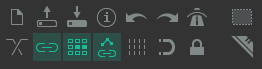
\includegraphics[scale=0.75]{user_guide_images/reaper_default_toolbar}
\par\end{centering}
\centering{}\caption{\label{Ripple-editing-per-track}\textquotedblleft Ripple
editing per-track\textquotedblright , \textquotedblleft Item edit
grouping\textquotedblright{} and \textquotedblleft move envelope points with
media items\textquotedblright{} engaged...}
\end{figure}


\subsubsection{Preferences }
\noindent\begin{flushleft} Some of these options are essential for the functions
to work as expected. Others are just recommended. \par\end{flushleft}

\subparagraph{Project > Item Fade Defaults }
\begin{itemize}
\item \begin{flushleft} \textsc{Enable} Create automatic fade-in/fade-out for
new items, length: 0:00.010 \par\end{flushleft}
\item \begin{flushleft} \textsc{Enable} Overlap and crossfade items when
splitting, length: 0:00.010 \par\end{flushleft}
\item \begin{flushleft} \textsc{Enable} Overlap and crossfade media when
finalizing razor edits \par\end{flushleft}
\end{itemize}

\subparagraph{Appearance > Peaks/Waveforms }
\begin{itemize}
\item \begin{flushleft} \textsc{Uncheck} Draw faint peaks in folder tracks
\par\end{flushleft}
\end{itemize}

\subparagraph{Appearance > Fades/Crossfades }
\begin{itemize}
\item \begin{flushleft} \textsc{Enable} When editing crossfades with the mouse,
use crossfade editor theme colors \par\end{flushleft}
\end{itemize}

\subparagraph{Appearance > Track Control Panels}
\begin{itemize}
\item \begin{flushleft} \textsc{Ensure} Folder collapse button cycles track
heights is set to `Normal, small, collapsed`. \par\end{flushleft}
\end{itemize}

\subparagraph{Appearance > Zoom/Scroll/Offset}
\begin{itemize}
\item \begin{flushleft} \textsc{Change} Offset by\dots percent of item height to
100\footnote{In REAPER versions prior to 6.54, these options don't exist.
Instead, under \emph{Appearances}, you need to change \emph{Maximum number of
lanes, when showing overlapping items} to 2} \par\end{flushleft}
\item \textsc{Check} Draw as opaque
\end{itemize}

\subparagraph{Editing Behavior}
\begin{itemize}
\item \textsc{Set }Locked item ripple editing behavior to `Locked items are
unaffected by ripple'\footnote{Technically not necessary as it is now checked
and set at the start of ripple-capable functions.}
\end{itemize}

\subparagraph{Editing Behavior > Mouse Modifiers}
\begin{itemize}
\item \textsc{Change }Razor edit area left drag default to `Move areas,
disabling ripple edit'
\end{itemize}

\subsubsection{Project Settings }
\begin{itemize}
\item \begin{flushleft} \textsc{Change} Video > Frame rate to 75\footnote{The
number of frames per second for red-book CDs.} \par\end{flushleft}
\item \begin{flushleft} \textsc{Change} Render resample mode to r8brain free
(highest quality, fast) \par\end{flushleft}
\end{itemize}

\subsubsection{Theme Tweak}
\begin{itemize}
\item \begin{flushleft} Using the ``Theme development: Show theme
tweak/configuration window'' action, search for ``mute'' and change the alpha
blend to 0.00. See figure \ref{Setting-mute-overlay}. \par\end{flushleft}
\item Set the super-collapsed value to 0 in rtconfig.txt. See figure
\ref{fig:Super-collapsed-value-is}.
\end{itemize}
\begin{flushleft}
\begin{figure}
\begin{centering}
\includegraphics[width=1\linewidth]{\string"user_guide_images/theme tweak\string".png}
\par\end{centering} \caption{\label{Setting-mute-overlay}Setting mute overlay
mode}
\end{figure}
\par\end{flushleft}

\begin{figure}
\begin{centering}
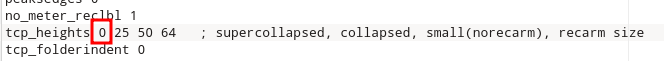
\includegraphics[width=1\linewidth]{user_guide_images/super-collapsed}
\par\end{centering} \caption{\label{fig:Super-collapsed-value-is}Super-collapsed
value is set to 0 in rtconfig.txt}
\end{figure}

\noindent\begin{flushleft} At this point it might be a good idea to Save as
default project settings as well as make a classical template (if you didn't
download mine) so that you don't have to do this setup more than once.
\par\end{flushleft}

\pagebreak
\includepdf{cover-back}
\end{document}
